\chapter{智能会话系统}{Toward Intelligent Dialgoue}

         本文研究的其中一个长远目标便是结合前文提到的各项自然语言处理和逻辑推理技术,构建一个能较好地与人交流沟通的智能会话系统,此系统将接收到的人类话语转化成逻辑表达形式,并且结合系统本身的动机和情感状态,经过一定的解析和逻辑推理,从而得到想表达的内容的逻辑表达形式,最后将这些逻辑表达式再转化成自然语言回应给谈话对象。

       本章将重点介绍这样的智能会话系统(以下简称“CogDial”)的系统架构,该系统基于前面章节描述的自然语言理解和自然语言生成的相关技术,并通过OpenCog的核心子系统(主要是PLN和OpenPsi)来控制其对话结构和表达方式。该CogDial系统能够灵活地理解和处理具有不同程度的复杂性和智能性的人类言语行为。创建一个完全符合人类标准的人工智能对话系统无疑是一个精彩的挑战,但似乎在当前的科学技术水平下,也无疑是一个非常困难的研究项目。 相对于目前主流的基于规则或者基于统计的对话系统,我们这里提出的CogDial架构引入目标驱动的逻辑推理和情感控制等,显然表现更智能些,但还不足以完全达到符合人类智能标准。这样一个介于目前相关研究水平和完全人类水平之间的对话系统可以看做是构建更人性化的对话系统的一个重要步骤,或者看做是使用更可行的研究方法在人机对话系统上集成更多的功能,而不是一味地去盲目追求达到人类水平的目标。本着这样的理念,说的更具体点,我们CogDial的目标不是精确类似人类的对话,而是具备通用认知能力、情感表达能力、能合理结合语用和经验的智能会话系统。

         CogDial的初步预期目标主要是实现面向游戏角色和人性机器人的对话系统,但同样的研究思路也完全能应用在基于文本的对话系统,例如智能对话搜索接口。我们分阶段来实现这样的系统,以一个相对小而简单的系统为起点,通过不断改进和完善,以及结合系统本身的自学习和认知能力,最终实现一个在一定程度上接近人类水平的系统。目前,我们的系统还没有达到最终的水平,但基本框架已经到位。除此之外,我们构建了一个基于超图匹配的问答系统的原型,该问答系统使用前文提到的自然语言理解技术将自然语言转换成以超图表示的语义逻辑形式,利用基于超图匹配的动态编程算法,从而在问答语料库中找到最适合问题的答案来响应用户查询。

\section{基于Psi的对话控制}{Applying the Psi model to Dialogue Control}

构建一个完整能运作的智能对话系统,除了需要前文提到的各项关键技术, 宏观规划(以下称为“Marcoplanning”)也是必不可少的部分。从言语行为理论来看,宏观规划可以看成是一个可以规划以下两点的工具:1)在哪个时间点发生哪些言语行为,2)使用哪些内容去封装这些言语行为。宏观规划更多的是从语用和推理方面出发,淡化语义或语法(或者音韵词汇等)的限制。

      CogDial智能对话系统中的宏观规划涉及到了OpenCog中的情感动机计算模型OpenPsi,因此,在本节我们会首先给出OpenPsi的高度概括,侧重于介绍其在自然语言会话系统中应用的可行性。

\subsection{Psi模型中的动机行为}{The Psi Model of Motivated Action}
       为了更好的解释OpenPsi,我们需要从Psi和MicroPsi谈起,Psi是由德国心理学家Dietric Dorner提出的情感认知动机理论模型 \cite{Dorner2002},将情感与智能体的需求和动机相联系。{\bf MicroPsi} \cite{Bach2009},是一个基于Psi理论的一个开源的智能认知体系结构,实现了Psi理论中的动机、情感以及智能的关联模型,并在一些实用控制应用以及简单虚拟世界里的智能体上进行测试。MicroPsi在全面性以及神经科学和心理学依据方面做得非常出色,但是该认知体系结构在可扩展性上存在不少问题, \cite{EGI1}中,有人认为,MicroPsi目前使用的算法在学习和推理上不大可能被扩展或规模化。

       OpenCog受Psi理论中的动机和情感模型的启发,借鉴了很多MicroPsi的基本实现方法,实现了类似的情感动机模型OpenPsi。虽然OpenPsi和MicroPsi在一定程度上很相似,但两者 还是存在着很大的不同。比如,两者使用了完全不同的知识表达方式, MicroPsi则使用了类似神经元的“quad”来表示知识,每一个quad包括5个神经元,其中一个是核心神经元,其他4个描述与核心神经元的“前/后”或者“部分/整体”等关系。OpenPsi使用了本文第三章中介绍的OpenCog的基于超图的知识表示,显然是一种更灵活和通用的知识表示方式。 MicroPsi目前还是注重底层的智能的实现,还未开始着手高层的智能处理,如自然语言处理和抽象逻辑推理。
在本节对Psi和MicroPsi的概述中,我们主要介绍其在OpenCog被应用的部分,主要是处理动机、行为和目标的框架模型。

Psi理论中的动机机制可参考图\ref{fig:Psi},从下往上看,不难发现Psi的动机机制从能激发智能体的需求出发。对于动物来说,该需求可以是食物、水、保护自己的孩子、社交需求、新鲜感等等;对于智能机器人来说,该需求可能是电源、 完整性(保护身体完整Integrity)、确定性(了解和熟悉环境的需求Certainty)、认知需求、心里成长等等;对于智能对话系统来说,该需求可以包括收集相关信息、取悦谈话对象、使会话保持新颖不枯燥等。
Psi理论特别指出了两种相当抽象的需求,并认为他们是心理学上的最基本需求 (参见图\ref{fig:Mod})

\begin{figure}[htb]
\centering
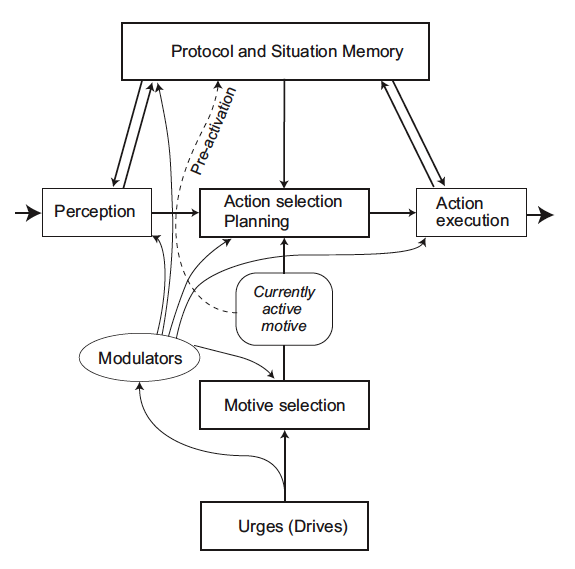
\includegraphics[width=11cm]{figures/Psi.png}
\caption{High-Level Architecture of the Psi Model}
\label{fig:Psi}
\end{figure}

\begin{itemize}
\item 能力需求(Competence):  智能体能有效实现某种强烈欲望的需求
\item 确定性需求(Certainty):智能体了解和熟悉环境的需求 
\end{itemize}

每种需求都有一定的偏好范围或目标范围,随着时间和环境(包括智能体自身)的不断变化,智能体的需求也在不断地变化。 当需求水平落在相应的目标范围时,
称作该需求被满足,否则需求不被满足。我们可以将智能体视为一个目标驱动的系统,其主要任务就是尽可能让所有这些需求都被满足。而当某一需求不被满足时,智能体会有一种试图将该需求水平恢复到偏好范围内的愿望,这种愿望便构成了{\bf 动机(Urge)}。


另外还有一种{\bf 愉悦感(Pleasure)}(和其反义的"不悦感")的原始概念,人们认为这种情绪与复杂的"幸福感"不同。愉悦感被解读成与愿望有关:当愿望(至少部分上)被满足,愉悦感便会由此而生;而当愿望愈趋强烈,不悦感则会由此产生。满足愿望的程度未必要被即刻定义;例如来说,它可被定义为一种需求对近期以来的目标范围随时间衰减的近似加权平均值。

因此,若智能体感到枯燥无趣,当受到大量新鲜感的刺激,它就会体验到某种愉悦感。若智能体感到枯燥无趣,而又更极端地受到单调的刺激,它就会体验到某种不悦感。

要注意的是,根据这相对简单的方法,任何幅度降低了不满感都会造成某种愉悦感;但若一切总是持续在其可接受的范围进行,就不会出现任何愉悦感。这看似有点违反直觉,但必须了解,这些简单的"愉悦感"与"不悦感"并不会完全掌握与这些字词相关的自然语言概念。此处使用的自然语言术语仅作为启发法传达涉及程序的一般特性。这些都是非常低水平的程序,在人类经验的相似情况远低于意识水平。
每个需求都有许多参数。如 Psi 模型所设,其中可调整的重要需求参数有:

\begin{itemize}
\item 权重:在特定时间点,相对于其他需求,该需求如何被加权
\item  增益:决定源自实现需求所得到的满足感多寡的定标因素
\item  损失:决定源自未实现需求所得到的未足之感多寡的定标因素
\item  衰减:基本上是被给定的愿望随着一段时间的增加率。

\end{itemize}

在此模型中,为刺激的缺乏使愿望随着时间增加。本人不确定这个模型是否与一般认知模型一样切实,但针对能确保某智能体持续在运作,这会是可行的短期机制。对应多种需求来调整增益、损失和衰竭等参数,便是变换智能体"个性"的一种方式。

接下来,{\bf 目标}被视为系统在未来某时间点致力成真的一种表达;而{\bf 动机}为一组 $(愿望, 目标)$配对,由一目标组成,该目标的满足感被预测隐含了某些愿望的满足感。事实上,愿望可被视为顶层目标(在 OpenCog 中有时又被称作 ”Ubergoals”),而智能体的其他目标则为子目标。"意图"也被视为综合体:在特定时间点的意图是由积极动机所构成,配合它们的相关目标、行为程序等。

在 Psi 模型中,智能体随时都有"主导动机";对 CogDial 的早期版本而言,虽然也是可行的假设,但大体上似乎是过度限制的假设,比起相似人类或其他高级人工智能系统,此假设或许更适合用在较单纯的模拟动物上。大致上可想成不同动机具有不同权重,而这些权重指出追求上所要耗费的资源量。

Psi 模型的基本行动逻辑是通过"三元祖"执行,非常类似 OpenCog 中的三元组$\textit{Context} \land \textit{Procedure} \rightarrow \textit{Goal}$ 。然而,有个重要角色是由四个调制因子扮演,其控制观感、认知和行动选择的程序如何在一特定时间受到规范:

\begin{itemize}
\item  活化度,决定智能体相对认知、反思活动,侧重于快速、密集活动的程度 
\item 分辨程度, 决定系统对于尝试解读世界的精准度 
\item 确定性,决定系统尝试达到确实、特定知识的努力程度 
\item 选择门槛,决定系统对改变其选择侧重的目标的意愿程度
\end{itemize}

这些调节因子在非常抽象的层次上表现出系统情绪和认知状态的特性;它们本质上并不是情绪,但它们对智能体的情绪有相当大的影响。它们预期的互动如图表\ref{fig:mod}所描述。


\begin{figure}[htb]
\centering
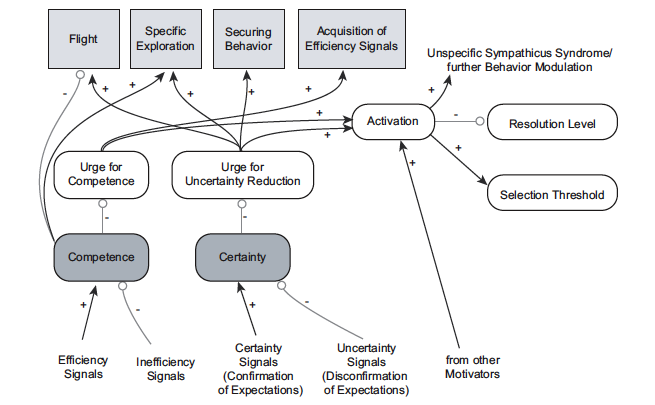
\includegraphics[width=12cm]{figures/PsiModulators.png}
\caption{Psi 调节因子之间的主要相互关系}
\label{fig:Mod}
\end{figure}

Psi 利用三个网络中安排的 Quad 储存知识,在概念上类似 Albus 的 4D/RCS 和 Arel 的 DeSTIN 结构:

\begin{itemize}

\item 储存陈述性知识的传感器网络:将图像、物体、事件呈现为分层结构的规划器 
\item 运动网络,通过阶层行为程序容纳过程知识
\item 处理需求的动机网络

\end{itemize}

Psi 模型的感知是根据 “HyPercept” 基于假设的感知的机制,其试图预测待理解的为何,并利用感知和记忆尝试验证这些预测。此外,根据对现实的探索和呈现之间的"Neisser知觉环",HyPercept 密切地联结外在世界的动作。感知上获得的信息会被转换为能够引导行为的规划器,再实施这些规划器(有时会显著影响世界),在进入用来引导进一步感知的程序。我们将不会利用 Psi 的这个层面,因 OpenCog 处理感知的方式不大相同。 
Psi 模型的动作选择是根据所谓的"三元组"运行,每个的组成是由

\begin{itemize}
\item 侦感器规划器(前置条件、"条件规划器";如 OpenCog 中的"语境")
\item 随后行动规划器(行动、效应器;如 OpenCog 中的"程序") 
\item 最终侦感器规划器(后置条件、预期;如 OpenCog 的谓语或目标)
\end{itemize}

区分这些三元组与用于 SOAR 和 ACT-R 中典型生产规则的不同之处,在于三元组可能不完整(三要素之中可能会缺少其中几个)且不确定。然而,在这三元组和 OpenCog 的概念/程序/目标三元组之间,似乎没有根本上的差异;MicroPsi 和 OpenCog 在此层面的差异,在于用于图解的基本知识呈现,以及用来表达含意的概率逻辑。
解出规划器待执行、以达到当前情境所选的目标,会在 Psi 模型中运用一种名叫"Rasmussen 阶梯理论"(以丹麦心理学家 Jens Rasmussen 之名命名)的程序结合来完成。Rasmussen 阶梯理论说明动作的组织,是这三种行为阶段的动作;其中有以技能为基础的行为、以规则为基础的行为和以知识为基础的行为:

\begin{itemize}
\item 若被给予的任务相当于训练过的例行程序,则会活化自动行为或技能;一般而言可不经由意识注意或慎重控制来执行。 
\item 若尚无自动行为,行动步骤可能会出自规则;在可采用一组已知策略之前,必须先对情况做分析,使策略适合用于情况。 
\item 若没有适用的已知策略,在这些情况下,必须先找出合并现有操作指令(运算元)到达成所设目标的方法。此阶段通常要求行为的重新构成,也就是规划的程序。
用于 Psi 和 MicroPsi 执行的规划算法是个相当简单的爬山法规划器。虽有人假设,针对高级智能也许会需要较复杂的规划器;但部分 Psi 模型的假设,是建立于一旦有机体具有正确的知觉表征和目标,大多数对该有机体进行实际规划所要做的,就相当简单。
\end{itemize}


在我们现使用的 CogDial 系统,如以下将说明的,为相应 Psi 模型中提及之前两种动作的认知规划器。某些感知规划器包含纯反射、自发行为(例如对"你好吗"的问题回答"我很好");其他则存有需要大量推理的行为。然而,目前 CogDial 的版本尚无法处理已知策略不适用的情况。大致上,OpenCog 确定会支持这种弹性情况,但我们仍在努力研究出有效运作于此对话语境中的更多基本行为。这是 CogDial 方法和纯发展性学习方法(这在 OpenCog 结构中也可能采取)之间的差异性;在效法人类幼童的认知和语言发展的发展性学习方法中,该基础在于处理已知策略不适用的情况,以及在此等情况下学习策略(虽有出生即具有相当高水平学习策略的论证,以及对多种有益于对话的行为之成见,但幼童并非一出生就具有任何处理对话情况的策略)。

%%%%%%%%%%%%%%%%%%%%%%%%%%%%%%%%
\subsection{Psi 模型中的情感与个性}{Emotion and Personality in the Psi Model}
%%%%%%%%%%%%%%%%%%%%%%%%%%%%%%%%

情感是人类心理学和人机交互的重要层面。若对话系统能够做到情感的自然互动,对人类谈话对象而言,自动化自然语言对话将更加受人注目且令人满意。要将情感自然度注入到对话中,Psi 模型会是合适的方法,因其含有栩栩如生的人类情感模型 。
Psi 中的情感被视为复杂的系统响应模式,而不是清楚构建出的实体。情感是响应某特定愿望所唤起的心理实体。在 Bach 的论文 \cite{Bach2012} "涌现的情感"(”Emergent Emotions”) 中,他将特定的情感与基本的调制器值建立关连,例如:

\begin{itemize}
\item 愤怒(Anger):负价、高激发性、低决断水平、选择阈值高
\item 伤心(Sadness):负价、低激发性、高决断水平、低防御度、低意图性 
\item 喜悦(Joy):正价、高激发性、低决断水平
\item 福佑(Bliss):正价、低激发性、高决断水平
\item 沮丧(Frustration):负价、中等激发性、低决断水平、选择阈值低(此为近期才加入到本文的研究中,而前面的项目则是出自前文提及之 Bach 的论文)
\end{itemize}

这类关系在概念上的性质或许值得强调。我们并不是在试图将人类的情感以任何意义上"降低"为调制器值的结合。确切的说,我们认为如"愤怒"、"喜悦"等情绪字词,都是对复杂的人类心理动力极原始的叙述。通过适当地合并调节器的值,我们就可经由许多情感字词所示的指出系统动力空间惯常上稍接近的区域。当然人脑/人体的动力系统含有许多未在 Psi 中建模的复杂参数,我们并不尝试做出精准无误的神经生理情感模型。
个性 – 在对话语境中也是个有趣的话题。若想创建显示多种个性特质的对话系统,可能要以密切相关的方式来处理。经典的人格"五大因素"模型,是使用五种因素来解释人类个性的变异:

\begin{itemize}
\item 直率性(openness)
\item 尽责性( conscientiousness)
\item 外向性 (extraversion)
\item 亲和性(agreeableness)
\item 情绪不稳定性(neuroticism)
\end{itemize}

"涌现的情绪"(”Emergent Emotions”)文中论证,这些至少可从增益、衰减和损失参数的角度粗略地解释归属感、竞争、确定性和美感等需求。 
基于这点,可根据多种需求的参数来撰写计算所设人物五大因素每项估计值的程式码。或者也可逆转数学,写出简单的等式,其中含有

\begin{itemize}
\item 输入:针对五大人格因素的量性度量,与特定人物相联系 
\item 输出:针对归属感、竞争、确定性和美感等需求的具体增益、损失和衰减参数值,意图相应于人格五大因素的指定的值
\end{itemize}

通过对每项人格五大因素(例如个性被指定为五维向量)从范围 [0,1] 指定一个数字,即可在建构档案中指定一人物的个性。当然与人类个性的错综复杂相比,这显然较粗糙;但针对适合的特殊应用情况,配合提供的对话系统个性内容,在合理程度上这会是很务实的工具。


%%%%%%%%%%%%%%%%%%%%%%%%%%%%%%%%
\section{OpenPsi:OpenCog中的基于Psi的动机性行为模型}{OpenPsi: Psi-Based Motivated Action in OpenCog}
%%%%%%%%%%%%%%%%%%%%%%%%%%%%%%%%

本节将介绍OpenCog中如何集成基于Psi的动机性行为模型,使其能为我们的智能会话系统CogDial提供能用于动机性行为选择机制。

%%%%%%%%%%%%%%%%%%%%%%%%%%%%%%%%
\subsection{OpenCog中的行为选择机制}{ Action Selection in OpenCog}
%%%%%%%%%%%%%%%%%%%%%%%%%%%%%%%%

正如Stan Franklin\cite{Franklin1995}指出的,智能的{\it 智能体}的本质在于它可以做事,还可以采取{\it 行为}。我们的智能会话系统CogDial中的行为选择会涉及OpenCog中所采用的行为选择机制\cite{EGI2},因此本章节首先简单介绍该行为选择机制的基本思路,以及Psi的变体模型如何在OpenCog中处理动机(包括情感、驱动、目标等)和对行为选择的指导。

OpenCog中的行为选择机制的关键部分在于:

\begin{itemize}
\item 行为选择器(Action Selector)根据当前环境选择可能帮助实现重要目标的程序
\begin{itemize}
\item {\it 例如:} 假设当前十分重要的目标是取悦谈话对象,一旦谈话对象问了问题,那么回答该问题会被评估为很可能可以达到“取悦谈话对象”的目标的程序。
\end{itemize}

\item 为了支持行为选择器,OpenCog设立了这样的蕴含式$Context \& Procedure \rightarrow Goal$,其中上下文(Context)是一个被赋值于智能体处境的谓词,在智能对话系统中,我们视为语境。

\begin{itemize}
\item {\it 例如:} 如果Bob请求智能体(智能会话系统)去写一段话,又假设该智能体知道Bob非常执着,那么该蕴含式可以被用成:
 \begin{itemize}
 \item ``Bob命令执行 X''  and ``执行 X''  $\rightarrow$ ``取悦 Bob''  $<.9,.9>$
 \end{itemize}

\item {\it 例如:} 如果智能体想说服谈话对象相信某个陈述X,那么该蕴含式可以被用成:
 \begin{itemize}
 \item ``告诉Bob我为什么相信X是正确''  and ``我想要说服Bob相信X是正确''  $\rightarrow$ ``满足度''  $<.9,.9>$
 \end{itemize}

\end{itemize}
\item 这些蕴含式的真值可以根据经验和推理来赋值。
\begin{itemize}
\item {\it 例如:} 第一个例子中的蕴含式的真值可以根据经验来赋值,即通过与记忆里Bob给出指令相关的情节来判断
\item {\it 例如:} 也能根据推理来赋值,即根据与Bob相似的个体给出指令的经验来类推,或结合Bob本人的明确表达,和Bob的自我描述通常合理的知识来推断
\end{itemize}

\item 重要值(Importance Value)可以通过经济注意力分配(Economic Attention Allocation)\cite{EGI2}在目标之间传播,推理可用于从现有目标中学习子目标。目前,这一点还未被利用在CogDial系统中,但我们相信这点能帮助实现更复杂的对话行为。
\begin{itemize}
\item {\it 例如:} 如果Bob告诉智能体去做X,那么智能体将“取悦Bob”的目标分解为“做X”,那么“取悦Bob”的目标会将它的重要值分给“做X”的目标(同样,“做X”的目标会将其重要值分给它的子目标,或者分给执行“做X”)。
\end{itemize}
\end{itemize}

%%%%%%%%%%%%%%%%%%%%%%%%%%%%%%%%
\subsection{Psi在OpenCog中的使用}{Psi in OpenCog}
%%%%%%%%%%%%%%%%%%%%%%%%%%%%%%%%

这里我们讨论Psi模型中的动机性行为的基本模块是如何被集成到OpenCog中的,更深入的了解,可参考文献 \cite{Zhenhua2011}中使用OpenPsi(即OpenCog中实现的Psi的情感和动机模型)来控制游戏世界里的动画角色。这里只简单地列出其中的实现要点


\begin{itemize}

\item 需求用GroundedPredicateNodes(GPN)表示,即节点的真值计算由一些内部的C++程序或者程序库中Combo程序来完成

\begin{itemize}
\item {\it 例如:} 警觉,外界感知的新鲜感,内在的新鲜感,得到老师的奖励,社交刺激等
\end{itemize}

\item 动机也用GPN表示,其真值根据需求所对应的节点的真值来定义。OpenCog中有时使用Ubergoal来代替动机(Urge),通常用来表示顶层目标。

\item 每个系统都有固定的Ubergoal集合(且只有非常高级的OpenCog系统可以修改它们的Ubergoals)

\begin{itemize}
\item {\it 例如:} 现在和将来都要活着并保持警惕;现在和将来都要经历和学习新的东西;现在和将来都要从老师那获得奖励;现在和将来都要和其他智能体都要有丰富的社交行为等

\item  一个更高级的OpenCog系统可以把有抽象(但必须与经验绑定)的伦理原则作为其中的Ubergoal。例如:根据 \cite{GoertzelHP}讨论的伦理道德, 一个Ubergoal是追求快乐;一个Ubergoal是促进成长;一个Ubergoal是帮助抉择
\end{itemize}

\item Urbergoal中的ShortTermImportance(STI)表明该目标的紧急程度,因此,如果对应Ubergoal的需求在其目标范围内,那么Ubergoal的STI值为0。所有的Ubergoal都能被给定最高的LongTermImportance(LTI),以保证他们不会被删除。

\begin{itemize}
\item {\it 例如:} 如果系统在一个(根据Ubergoal)持续提供足够的新鲜感的环境里,那么对应外界新鲜感需求的Ubergoal会有低得STI值但是高的LTI值,表示该系统不会浪费资源在寻求新鲜感上。但如果环境变得更单调,那么对外界新鲜感的需求的紧急程度就会增加,而其中的STI也会相应增加,资源会开始重新分配在提高新鲜感上

\end{itemize}

\item 愉悦感也是用GPN表示, 其中的内在真值计算程序将Ubergoal的满足度当成其期望的满足度。

\begin{itemize}
\item 有多种数学函数能用于平均不同Ubergoal的满足度(针对不同$p$的$p'th$ power averages\footnote{the $p'th$ power average 可定义为 $\sqrt[p]{\sum X^p}$} for different $p$),而这里对愉悦感的不同计算方式的选择,可以带来不同“个性”的系统。

\end{itemize}

\item 目标可以用节点或边来表示。系统的目标列表被称为目标池(Goal Pool)。Ubergoal一般都是自发性的目标,但也有可能有许多其他目标。

\begin{itemize}
\item {\it 例如:} “从老师那获得奖励”的Ubergoal可以产生类似“从Bob那得到奖励”(如果Bob是老师)的子目标,也可以产生“使老师微笑”,或“创造新的令人惊讶的话语”(如果后者也能得到老师的奖励)的子目标
\end{itemize}

\item Psi中记忆使用OpenCog中的知识库Atomspace来表示
\begin{itemize}
\item {\it 例如:} OpenCog智能体在什么语境下说过什么的记忆都会存储在Atomspace中。

\item 在Psi和MicroPsi中,同样的现象会以完全不同的表达方式存储在记忆空间中,但Psi的基本动机模型与这些存储方式无关。

\end{itemize}

\item Psi的动机选择在OpenCog中通过经济注意力分配(economic attention allocation)来执行,即对目标节点分配ShortTermImportance  

\begin{itemize}
\item {\it 例如:} 重要值从“从老师那得到奖励”到“从Bob那得到奖励”到“给Bob讲个笑话”的传播流程,是Psi中被称为“动机选择”的一个实例。虽然还没开始执行任何行为,但智能体在这过程中已经对该实现哪个的具体目标做出了选择,而这个具体目标会被用于指导行为的选择。
\end{itemize} 

\item Psi的行为选择被用于OpenCog的行为选择,但在OpenCog中,行为选择的问题就是选择哪个{\it 程序}(即“规划器(schema)” )去执行,而不是选择哪个具体行为去执行。其实,类似的概念在Psi上也存在,Psi中的“自发性行为(automatized behaviors)”类似OpenCog中的规划器;唯一的区别就是在OpenCog中这些自发性行为是默认的情况。

\begin{itemize}
\item {\it 例如:} 如果“做一个能惊讶谈话对象的有趣声明”有一个高的STI,那它可被用于激励相关执行程序的选择。如“从以前读过的文本里找到有趣内容,从中抽取摘要,并简明地表达这些摘要”的程序。 当一个程序被选择时,该程序还可能触发相关的子程序的执行。
\end{itemize}

\item Psi的规划通过OpenCog中的多种学习过程来实现。大部分的学习过程通过逻辑推理引擎PLN来完成(也是本文目前关注的学习机制),还可以通过OpenCog中的遗传编程工具MOSES或者爬山算法等来实现。
\begin{itemize}
\item {\it 例如:} 当智能体决定说服谈话对象相信某事实X时,它可能需要进行周密的计划,如:推断出谈话对象缺少哪些相关的背景知识去理解X,然后首先给谈话对象传输所缺的相关知识,再来传输X。

\end{itemize}

\item 调节因子用系统参数表示,可以用PredicateNode来表示,且必须在多个动态的MindAgents之间相互协作。如:
\begin{itemize}
\item {\it 激活度(activation)} 影响行为选择。当激活度较高时,智能体倾向于做出快速响应外部刺激,因此可能会选择那些能做快速回答的规划器来执行。
\item {\it 解析度(resolution level)} 影响推理。当解析度较低时,智能体选择减少精力去解析输入中的语言现象。
\item {\it 明确度(certainty)} 影响推理、模式发掘以及新概念构建的过程。当明确度较低时,智能体接受更多不确定的结论。
\item {\it 选择阀值(selection threshold)}引入偏好信息,可以帮助智能体在几个互相冲突的目标之间做出选择。
\end{itemize}
\end{itemize}

%%%%%%%%%%%%%%%%%%%%%%%%%%%%%%%%
\subsection{OpenCog中的目标}{Goals in OpenCog}
%%%%%%%%%%%%%%%%%%%%%%%%%%%%%%%%

OpenCog中,一个目标Atom表示 一个\textit{目标系统状态},当系统在一定程度上满足了其表示的条件,那么该目标Atom的真值就高;一个上下文Atom表示 \textit{已经观察到的状态} ,当定义的状态都被察觉,那么该上下文Atom的真值就高。这两个Atom类型构成了那些需要在特定的上下文环境下实现具体目标的OpenCog系统的基础。但也不是所有OpenCog的行为活动都需要这两类型的Atom来指导,尤其是那些自发的,不面向目标的任务。

具体实现上,一个目标Atom是被GoalRefinement的MindAgent挑选出来的系统认为很需要被实现的Atom(通常式一个PredicateNode,有时是边,也有可能是其他类型的Atom)。GoalRefinement通过调用RFS (Request For Service)来及时确定某Atom是否能被当成目标Atom。

一个OpenCog的实例必须从初始的 \textit{Ubergoals}(即\textit{顶层目标})开始,但可以多种推理方式去细化这些顶层目标。相对简单的,或者只关注某个应用的OpenCog系统不能修改自己的顶层目标,也不能添加或删除顶层目标。但高级的OpenCog系统有权限修改、添加或删除顶层目标,但这些操作对系统的动态机制有着很关键和不易察觉的影响,必须谨慎对待。

\paragraph{目标组建}\label{Goal Formation}

除了初始设定的Ubergoal之外,OpenCog中还可以通过PLN推理来组建新的目标。概括地说,PLN通过推理查找那些能在一定概率上蕴含现有目标的谓词,来进行新目标的组建。这些谓词一旦被用于新目标组建后,会被赋值更高的注意力值,那么根据OpenCog的目标驱动的注意力动态分配机制可知,这些新目标会触发系统中能满足它们的相应程序。

下面通过一个从ExternalNovelty(外在新鲜感)的Ubergoal开始组建子目标的例子来说明OpenCog中如何细化目标。假设该智能体已经学习到,每次Bob给它读诗的时候,它的外在新鲜感能在很大程度上得到满足,也就是说:

\begin{verbatim}
Attraction
   Evaluation recite (Bob, me, poem)
   ExternalNovelty
\end{verbatim}
\noindent 其中,$\textit{Attraction}\ A\ B$ 衡量 $A$ 蕴含B高于$\lnot A$蕴含B的程度。

这些信息允许智能体指定以下的Atom:

\begin{verbatim}
EvaluationLink recite (Bob, me, poem)
\end{verbatim}

\noindent 为一个目标(Ubergoal的子目标)。这是一个如何细化目标的实例,也是PLN从现有目标中创建新目标的多种方式中的一种。

\paragraph{OpenCog中的上下文环境}\label{Context Atoms}

最简单的情况下,上下文环境可以被简单地看成是一个ContextLink的内容来源,例如:

\begin{verbatim}
Context
    quantum_physics
    Inheritance Ruiting amateur
\end{verbatim}

%%%%%%%%%%%%%%%%%%%%%%%%%%%%%%%%
\subsection{管理的执行}{Execution Management}
\label{Execution Management}
%%%%%%%%%%%%%%%%%%%%%%%%%%%%%%%%

被命名为GoalFulfillment的MindAgent会选择可以实现当前目标的规划器,但并一定执行这些规划器,而是将这些根据当前目标选择得到的规划器放入ActiveSchemaPool中,对于ActiveSchemaPool中的每一个规划器$S$ ,都能满足具有较高真值的:

\begin{verbatim}
Attraction
   C
   PredictiveAttraction S G
\end{verbatim}

其中$C$表示当前可用的环境,$G$是目标池中的某个目标。

当SchemaAction启动时,该MindAgent会调用ExecutionManager来决定执行ActiveSchemaPool 中哪个规划器。ExecutionManager根据推理以及查询记忆知识,选择那些不会同时引起\textit{破坏性干扰}(且希望能引起建设性影响)的规划器来执行。该过程可能(间接地)会导致新的规划器的创建,或者Atomspace中的其他规划器被激活。


%%%%%%%%%%%%%%%%%%%%%%%%%%%%%%%%
\section{智能会话系统CogDial的架构}{The CogDial Dialogue System Architecture}
%%%%%%%%%%%%%%%%%%%%%%%%%%%%%%%%

下面我们来介绍基于上述的目标控制体系的智能会话系统CogDial的系统框架。目前该系统只能处理英文对话,接下来章节中的对话的例子基本按照英文的习惯举的例子,可能不太适合中文的习惯,但是该系统的所采用的技术和理论基础都是完全适合中文的。CogDial主要采用了以下技术:

\begin{itemize}
\item  基于OpenPsi以及相关OpenCog机制的宏观规划(Macroplanning)
\item  本文第4章描述的句法分析和语义关系及逻辑关系抽取的自然语言理解技术
\item  本文第5章描述的微观规划(Microplanning)和表层生成的自然语言生成技术
\item  专门设计的符合智能会话系统的“言语行为规划器”集合,这些言语行为规划器将用于:
\begin{itemize}
    \item 在OpenPsi的控制机制下,结合当前的语境,激活相应的言语行为规划器
    \item 收集相关内容,生成能关联Microplanner的Atoms
    \item  调用一系列的认知机制(包括用于逻辑推理的PLN),选择相关的Atoms发送到Microplanner
\end{itemize}
\end{itemize}

%%%%%%%%%%%%%%%%%%%%%%%%%%%%%%%%
\subsection{针对对话控制的OpenPsi的配置}{Configuring OpenPsi for Dialogue Control}
%%%%%%%%%%%%%%%%%%%%%%%%%%%%%%%%

基于Psi的基本框架,我们选择了以下的具体需求用来指导我们的对话系统的行为:
\begin{itemize}
\item 社交需求(Affiliation):与他人互动,希望被其他成员接纳的需求;取悦谈话对象可以视为此目标的一个特例
\item 能力需求(Competence):通过对话达到某种目标的需求,衡量言语表达方式的指标
\item 确定性需求(Certainty):智能体对自身语境的了解需求,特别是对目标的了解需求
\item 新颖性需求(Novelty):维持智能的会话而不是简单重复的问答会话。
\end{itemize}

CogDial中的对话控制主要通过不同的需求来选择相应的言语行为规划器,因此,在选择言语行为规划器前,我们需要知道当前状态下上述每种需求的被满足的程度。鉴于目前的CogDial系统的有限能力,为了能更好地实现一个面向集成认知体系的智能会话系统框架,我们将上述的几项需求做了更具体化的定义:

\begin{itemize}
\item 社交需求(Affiliation):我们对该需求进行了下面三种满足程度:
\begin{itemize}
\item 当对话系统正在与人或者其他智能体进行会话时,该需求在一定程度上被满足;
\item 当系统正与多个人或智能体进行会话时,该需求被满足的程度提升;
\item  当该系统的会话内容都属于积极向上的时候(通过情感分析技术实现),该需求被满足的程度达到最高。
\end{itemize}
\item 能力需求(Competence):此项需求需要通过OpenCog来评估。简单来说,对每一个目标,OpenCog记录着会话系统在过去完成该项目标的程度,然后根据当前的不同目标所占的权重,我们可以通过以下公式估算该需求被满足的程度(首先针对每一个目标,计算目标权重*能达到该目标的概率,然后求总)。当然计算目标被完成的程度,还应该考虑实现目标的语境等因素,目前我们的系统更注重构建一个智能会话系统框架,因此在语境无关的假设下来衡量目标被实现的程度。
\item 确定性需求(Certainty):如果会话系统正在和一个陌生人对话,或者系统无法理解大量被提及的单词或概念,那么当前的确定性需求被满足的程度就会降低。如果系统获取了新的可靠知识,那么该需求被满足的程度就会增加。
\item 新颖性需求(Novelty):我们定义了以下几种方式来增加智能绘画系统对新鲜度需求的满足程度值:
\begin{itemize}
\item 多和不同的人类或智能体会话;
\item 谈论新的话题或引入新的词汇和概念;
\item 学习新的可靠信息( OpenCog推理得出的新的置信度高的知识存储的载体原子(Atoms))
\end{itemize}
\end{itemize}

基于上述目标需求的智能会话系统,除了需要结合前文所述的OpenPsi的框架理论,以及本文描述的自然语言理解和生成的相关工具之外,还需要有以下模块:
\begin{itemize}
\item 制定一组能被特定目标需求激活的对话控制程序
\item 建立目标和相应去实现目标的行为之间的关联,可通过相关规则来实现,也可以通过强化学习来实现,我们系统框架采用两种结合的方法,但目前的系统还是以规则关联为主。
\end{itemize}
  

%%%%%%%%%%%%%%%%%%%%%%%%%%%%%%%%%%%%%%%%%%%%%%%%%%%%%%%%%%%%%%%
\subsection {言语行为规划器}{Speech Act Schema}
\label{sec:SAS}
%%%%%%%%%%%%%%%%%%%%%%%%%%%%%%%%%%%%%%%%%%%%%%%%%%%%%%%%%%%%%%%

“言语行为规划器”(Speech Act Schema)是CogDial的一个核心设计, 每个言语行为规划器里包含一种特定的言语行为(Speech Act),以及与该言语行为对应的特定的认知行为(Cognitive Procedure)。每种言语行为规划器都能在不同情况下被激发调用。对于言语行为规划器的选择,我们采用OpenCog中的OpenPsi的动机驱动模块来执行。

    CogDial的总体规划是针对本文第 \ref{chap:litreview}章综述里提到的42种SWBD-DAMSL言语行为 \cite{Twitchell2004},实现相应的言语行为规划器。 CogDial目前只实现了42种中的部分言语行为对应的言语行为规划器。另一方面,CogDial中的言语行为规划器的设计也绝不局限于这42种言语行为,CogDial实现了一些言语行为规划器能对应这42种中的某两种或多种言语行为,比如我们利用真值回答规划器(TRUTH VALUE ANSWER schema)来同时关联其中的YES QUESTION和NO QUESTION,从而可以将一般疑问句的回答根据真值的大小延伸到“可能”“不确定”“可能不”等,而不仅仅是局限于回答“是”或者“不是”。CogDial还根据智能体的具体情况拆分了这42种中的某些言语行为,例如,我们针对言语行为“STATEMENT” 实现了两个不同的言语行为规划器:回应声明以及智能体自发的用于表达其自身状态和想法等的声明。

总的来说,本文虽然没有完全照搬SWBD-DAMSL的言语行为分类,但是,该分类体系是来源于对大量人类会话的进行具体分析后的实验结果,也在具体的会话分析和抽象的言语行为理论之间架起了桥梁,使得抽象的言语行为理论在机器上实现变得可行,因此,SWBD-DAMSL的言语行为分类体系还是很有借鉴价值的。

要实现上述的言语行为规划器,每一个言语行为都会引发一个相应的认知行为,也就是说,每一个言语行为都会触发调用一段程序;而这样的机制正好符合OpenCog里的 GroundedSchemaNode的用法。GroundedSchemaNode是OpenCog的超图知识库里的一种节点类型,通常被封装在ExecutionOutputLink里,连接着一段代码(一般情况下是Scheme或者Python编写的代码)的名称。该代码可以通过ExecutionOutputLink被触发和执行。因此,鉴于这样的执行机制,我们可以通过对每个言语行为规划器定义一个GroundedSchemaNode来实现言语行为规划器。这样的设计方案可以减少冗长复杂的代码块,而直接通过OpenCog中统一又通用的Atomspace的基本操作方法来管理和执行复杂的言语行为规划器。另外,这样的机制也能很容易调用知识库Atomspace之外的复杂程序,从而得到很好的扩展性,也为言语行为规划器的扩展研究搭建了个很好的平台。例如,我们可以通过调用外部程序将逻辑推理系统PLN的前向或者后向推理应用到言语行为规划器中,使其能实现自适应学习,不断完善言语行为规划器。本文后面会进一步讨论这样的扩展。

每一个言语行为规划器的输入是一个被叫做对话节点(DialogueNode),DialogueNode是可以表示一方或者多方之间的会话交互的节点类型。DialogueNode可以有不同话语节点(UtteranceNodes)作为成员,在实现方式上,DialgoueNode通过MemberLinks指向不同的UtteranceNodes。而UtteranceNode则可以关联以下不同类型的节点:
\begin{itemize}
\item 关联一个或多个文本节点(TextNode)、句子节点(SentenceNode)或者短语节点(PhraseNode),则表示输入的话语内容来自一个或者多个文本、句子或者短语。
\item  关联一个声音节点(SoundNode),则表示该话语来自外界声音。
\item  关联指向说话者的Link。
\item  关联指向对话语的补充信息的Links,这些补充信息可以是该话语的言语行为类型、与该话语相联系的情感等。
\item  关联指向产生话语的言语行为规划器,用于响应是什么触发该话语。
\item  关联一个或多个解析节点(InterpretationNode),这些解析节点可以是用来解析话语的语义和语用信息。
\end{itemize}

言语行为规划器的输出是连接了一系列相关联Atoms的SetLink,该输出会送入本文\ref{chap:generation}中描述的微观规划和表层生成等工具,从而产生相应的自然语言来回应输入的内容。言语行为规划器还会将输出的话语关联到产生该话语的DialogueNode,这样不仅仅是记录了会话的内容,还能用于智能体的强化学习和提高智能体的各种需求的满足度。
下面通过一个例子来解释上述的实现过程。假设有下面的简单对话:
\begin{verbatim}
Ruiting: How are you doing?
CogDial: I am fine
\end{verbatim}
这个简单的对话可用以下的Atoms来表示:

\begin{verbatim}

MemberLink
	UtteranceNode [555]
	DialogueNode [123]
	
MemberLink
	UtteranceNode [666]
	DialogueNode [123]
	
EvaluationLink
	PredicateNode "say"
	ConceptNode "Ruiting"
	UtteranceNode [555]

EvaluationLink
	PredicateNode "say"
	ConceptNode "me"
	UtteranceNode [666]
		
EvaluationLink
	PredicateNode "Textual Content"
	UtteranceNode [555]
	SentenceNode "How are you doing?"
	
EvaluationLink
	PredicateNode "Textual Content"
	UtteranceNode [555]
	SentenceNode "I am fine."
	
EvaluationLink
	PredicateNode "Utterance Type"
	UtteranceNode [555]
	ConceptNode "Interrogative"
	
EvaluationLink
	PredicateNode "Utterance Type"
	UtteranceNode [666]
	ConceptNode "Declarative"
	
AtTimeLink
	UtteranceNode [555]
	TimeNode "22:15:33 12/06/2014"
	
AtTimeLink
	UtteranceNode [666]
	TimeNode "22:15:47 12/06/2014"
	
EvaluationLink
	PredicateNode "Interpretation"
	UtteranceNode [555]
	InterpretationNode [22]
	
EvaluationLink
	PredicateNode "Interpretation"
	UtteranceNode [666]
	InterpretationNode [33]
	
	
MemberLink
	EvaluationLink
		PredicateNode "doing"
		ListLink
			ConceptNode "you"
			VariableNode "var1"
	InterpretationNode [22]
	
	
MemberLink
	InheritanceLink
		ConceptNode "I"
		ConceptNode "fine"
	InterpretationNode [33]
	
ExecutionLink
	GroundedSchemaNode "polite_banter.scm"
	ListLink
		UttteranceNode [555]
		DialogueNode [123]
	UtteranceNode [666]

\end{verbatim}

其中的命题也可以有多种选择,例如:

\begin{verbatim}
EvaluationLink
	PredicateNode "Conversation Partner"
	DialogueNode $D
	$X
\end{verbatim}

该命题为真,当且仅当,$X是$D其中一个话语的发言人。


\section{Initial Speech Act Schema and their Linkage to Goals and Contexts}{Initial Speech Act Schema and their Linkage to Goals and Contexts}

在\cite{Twitchell2004}, 中,Twitchell和Nunamaker根据Searl的言语行为理论的经典分类,在对大量的人类会话进行经验分析后,将言语行为细分为42种。虽然此分类体系很有理论研究价值,但在实验过程中,考虑到实用智能会话系统的语境等因素,我们对这42种言语行为做了稍微调整,同时也在CogDial中添加了一些SWBD-DAMSL研究中没有出现言语行为。

即使在有明确的言语行为类型的情况下,仍然有很多种方法去构建一个智能会话系统。CogDial根据多个广泛的可扩展目标制定一些特定的设计决策,在这些决策基础上,系统能通过自适应学习方法自动改进,为能跳出传统的对话系统的研究方法搭建一个基础平台。为了搭建这样的系统,需要考虑的第一点是,对于每一个言语行为,都有相应的固定形式的认知内容被触发,也有相应的习惯性表达方式来表达该认知内容。

如果在类似的言语行为类型分类基础上构建一个简单的“聊天机器人”,一般通过更简单,不用加入很多认知处理,针对每个言语行为类型,输出直接的具体的话语,也同样能达到类似的效果。例如,对于言语行为类型Agree,可以编写简单的程序使智能体输出“同意(Agree)”或者“是的,我同意(Yes, I agree)”。目前,“聊天机器人”的概念很模糊。我们这里提到的“聊天机器人”范围也很广,可以是完全基于模板匹配的聊天机器人ELIZA\cite{Weizenbaum1966},也可以是具有一些推理能力但是基本忽略语义理解的众所周知的Siri。但关键的一点是,我们设计的CogDial系统,是本着该系统能“理解”自己在说什么的理念,也就是说,该系统所产生的话语来自于内部的语义关系图,且该语义关系图和系统知识库中的其他语义关系图之间有着丰富的语义关系。我们希望系统能在一定程度上更深地“理解”自己在说什么,而不是只生成它不理解的字符串。在某些情况下,在不理解的情况下破口而出一些话语,尤其是习惯用语,也是可以接受的(其实人类有时候也会无意识地这么做),但这并不是大部分情况。

在CogDial系统的设计中,每一个言语行为都需要下列几项内容与之相应:
\begin{itemize}
\item 相应的目标和语境二元组(goal,context),表明何时该言语行为会被触发。
\item 相应的能生成相关信息的程序,产生由该言语行为引起的要传递给谈话对象的信息。
\item 一个或多个相应的“语义模板”,表明由该言语行为引发的相关认知内容。
\item 连接上述语义模板所在的Atoms和特定的句子实现的Atoms的Links,用于传送到Microplanning,从而生成相应的话语。
\end{itemize}

这样一来,通过编写一些抽象的语义形式和特定的会话习惯之间的匹配模式,便能构建出一个具有一定合理功能的智能会话系统,当系统学习了用不同的更复杂的表达方式去实现抽象的语义形式后,也就能在更大程度上“理解”会话内容。此外,这些抽象的语义形式除了与言语行为和目标需求相关联,还和其他不同的认知内容相关联,因此,系统会随着经验的增长而趋向成熟。
假设任何言语行为被触发都能增加下面表达式中的EvaluationLink的真值:
 \begin{verbatim}
EvaluationLink
	PredicateNode "Currently Having Conversation"
	TimeNode T
\end{verbatim}
    其中,“T”表示当前时间。又假设上面表达式中的EvaluationLink和系统中多个顶层目标有关联(该假设对于某些应用也不总为真,那么在这样的情况下,这些不为真的关联的链的权重会根据具体情况被调为适当的值),也就是说,该系统能看到会话行为带来的价值。 因为每个言语行为都蕴含着这个EvaluationLink,所以每个言语行为都会影响系统的目标实现。一些言语行为会通过持续进行对话从而超标完成某个系统目标。这样的言语行为会在后面章节详述。
    下面会给出一些具体的例子进一步解析前面几段提到的Atoms。
 \begin{verbatim}
ImplicationLink <.5>
	EvaluationLink
		PredicateNode "Currently Having Conversation"
		TimeNode $T
	EvaluationLink
		PredicateNode "Increase Knowledge"
		TimeNode $T
\end{verbatim}
上述超图片段表明,维持对话能在一定程度上满足系统目标“增长知识”,ImplicationLink的初始权重设为0.5,表明“当前有会话”蕴含系统目标“增长知识”只有0.5的概率。这个权重会随着系统的经验而改变,也会通过其关联的其他节点和链的具体情况推算得来。例如:
 \begin{verbatim}
ImplicationLink <.1>
	ANDLink
		EvaluationLink
			PredicateNode "Currently Having Conversation"
			TimeNode $T
		EvaluationLink
			EvaluationLink "DialoguePointer"
			PredicateNode "Currently Having Conversation"
			DialogueNode $D
		EvaluationLink
			PredicateNode "Conversation Partner"
			ConceptNode "Bob"		
	EvaluationLink
		PredicateNode "Increase Knowledge"
		TimeNode $T
\end{verbatim}

上面的超图片段表明,当进行对话的对象是Bob的时候,只有0.1的概率能实现系统目标“增长知识”。
\begin{verbatim}
ImplicationLink <1>
	ExistsLink $G, $S, $O, $U, $D
		ANDLink
			MemberLink
				GroundedSchemaNode $G
				ConceptNode "Speech Act Schema"
			AtTimeLink
				TimeNode $T
				ExecutionLink
					GroundedSchemaNode $G
					$S
					$O
			MemberLink
				UtteranceNode $U
				DialogueNode $D
			EvaluationLink
				PredicateNode "Textual Content"
				UtteranceNode $U
				SentenceNode $O
			AtTimeLink
				TimeNode $T
				EvaluationLink
					PredicateNode "Currently active"
					DialogueNode $D			
		EvaluationLink
			PredicateNode "Currently Having Conversation"
			TimeNode $T
\end{verbatim}

上面的例子说明,如果一个言语行为规划器被执行,当前的对话节点(DialogueNode)$D$会关联一个谓词“当前活跃”,表明$D$出于活跃状态, 那么“当前有会话”的目标被实现。

 \begin{verbatim}
MemberLink
	GroundedSchemaNode "answer_yes.scm"
	ConceptNode "Speech Act Schema"
\end{verbatim}

接下来的例子演示了言语行为如何与目标关联:

 \begin{verbatim}
ImplicationLink <.8>
	ExistsLink $S, $O, $U, $D
		ANDLink
			AtTimeLink
				TimeNode $T
				ExecutionLink
					GroundedSchemaNode "answer_yes.scm"
					$S
					$O
			MemberLink
				UtteranceNode $U
				DialogueNode $D
			EvaluationLink
				PredicateNode "Textual Content"
				UtteranceNode $U
				SentenceNode $O
			AtTimeLink
				TimeNode $T
				EvaluationLink
					PredicateNode "Currently active"
					DialogueNode $D			
		EvaluationLink
			PredicateNode "Please Conversation Partner"
			TimeNode $T
\end{verbatim}

上面的例子表明言语行为规划器“肯定回答”(”Answer Yes”schemma)可以用于增加实现“取悦谈话对象”目标的幅度值,超越了谈话对象因单纯继续对话而被取悦的程度。

许多言语行为规划器都会有不同的清晰表达相关语义内容的方式。比如说,一般会话的开头,可以说“你最近状态怎么样?”(”What has your state been recently?”),或者“你最近都忙什么?”(“What have you been doing?”) 等,而类似这样的语义内容很容易约定俗成地被说成“最近怎么样?”(“What’s up?”)。对于机器来讲,如果对话系统直接问 “What’s up?” 当然也没问题,但是有必要使系统知道 “What’s up?”只是其他两种说法或者 “what are you thinking about?“的一种约定俗成的简约说法。系统会根据智能体的不同个性对每种不同的说法一个相应的权值。

一般来说,会存在很多的“个性参数”影响着多种言语行为。在CogDial的实现过程,我们针对那些对对话影响较大的关键特性(我们称为“对话特征”(Dialogue-trait))创建相应的概念节点(ConceptNode),比如:习惯用语(Idiomaticity)、非正式(Informality)、精确(Precision)、累赘(Wordiness)、开放(Openness)。用来表示由言语行为规划器产生的具体话语的SetLink,将以不同的权重与这些表示不同对话特征的ConceptNode相连。例如,表示“I dunno”的SetLink将以较高的权重与“Informality”以及“Idiomaticity”关联,以较低的权重与“Precision”“Wordiness”关联。这些对话特征的参数可以在对CogDial设置基本参数的时候根据不同的需求人为设计。也可以在对话过程中根据谈话对象的喜好来自适应地调整。

综上所述CogDial的整个设计方案中,需要人工参与的部分包括:
\begin{itemize}
\item 自然语言理解流水线中的提到的规则(最终会被我们正在研究的无监督语言学习所取代,本文第9章有更详细的阐述)
\item OpenPsi中的顶层目标
\item 不同的言语行为所引发的不同认知过程。目前这些过程是在与GroundedSchemaNode绑定的相应Scheme或者Python代码中被实现。这些认知过程也可以在OpenCog的知识库Atomspace里被实现(如下文中的Question-answering schema)。
\end{itemize}
本章接下来的部分将进一步阐述CogDial使用的一系列言语行为规划器以及解释它们在CogDial中的实现机制,这些言语行为规划器大部分从SWBD-DAMSL中借鉴。当然这些特殊的言语行为规划器的集合并非一成不变,在以后对系统的不断改进和完善过程中,无疑会导致对该集合一定程度的延伸和细化。但我们相信这是一个好的开始,需要重申的是这些言语行为规划器分类是大量人类对话的实证分析的结果。目前,我们的研究工作重点在问答式规划器(Question-answering schema),将会在\ref{sec:QA}中进一步阐述。

\subsection{谈话开场白、结束谈话和转移话题}{Opening, Closing and Transitioning}

\begin{itemize}
\item 被放弃或转移、结束
\begin{itemize}
  \item 例如:"所以,嗯…"(”So, hmmmm....”)
  \item 相关目标、语境:当前谈话不尽能达到智能体的目的;但其中一些与谈话对象的对话,似乎仍有达到智能体目的合理程度上的可能性。或者,智能体无法想到任何与谈话对象所讲之相关的答复。当持续对话被断定为可达到智能体的某些目的,然而其他言语行为似乎无法在显着程度上充分达到智能体之目的;或当言语行为极有可能达到智能体的目标,然而看似与先前的对话失去连结性,在这样的情况下,这就会被使用(因此,某些言语标志对于划定新的谈话阶段之界线,是很恰当的)。
  \item 程序:在此情况下,待给予的语意内容往往会是"或许我们该来谈点别的"(”Perhaps we should talk about something else”)丶或"现在来谈谈别的吧。"(”Let us now talk about someone else”) 这样的语意内容会搭配清晰的咬字,也涉及社交上常见的言辞,比如"嗯…这个嘛…"(”Hmmmm... welll...”)。
\end{itemize}
\item 常见谈话开场白
  \begin{itemize}
  \item 例如:"最近过得怎样?"(”How’s it going?”)
  \item 相关目标、语境:一名潜在交谈对象在现场,经断定,与该对象交谈将能达到系统的目标。
  \item 程序:"常见谈话开场白"的性质,会以表示问候丶欲进行交谈的一种社会成规作为开端。有些常见的谈话开场白非常普通,例如"嗨。"(”Hi.”) 而其他较有语意内涵的,比如"现况如何?"(”What is your current state?”)丶"最近经历了哪些事?"(”What have been your recent experiences?”)丶"在想些什么?"(”What are you thinking about?”)丶"目前在从事些什么?"(”What are you involved with currently?”) 这样的语意内容会搭配清晰的咬字,也涉及社交上常见的言辞,比如"最近怎样?"(”What’s up?”)丶"有什么新鲜事?"(”What’s new?”)丶"生活怎么样?"(”How’s it going?”) 等。同样地,也可能会明白地问丶或通过惯用语表达"我想和你谈谈"(”I would like to talk to you”) 或"想聊天吗?"(”Would you like to chat?”) 等语意内容。 
  \end{itemize}
\item 结束谈话
  \begin{itemize}
  \item 例如:"那好吧…今天跟你聊天很开心。"(”Alrighty then... it’s been good to chat with you.”)
  \item 相关目标、语境:如结束谈话会是达成系统目标的最佳方式,这样的话语是很适当的。若确定谈话对象欲结束谈话,在这种情况下,结束谈话会是达成系统目标取悦谈话对象最好的办法。在任何情况下,比起唐突结束,用言辞结束谈话反而是达成取悦人类的目标最佳的方式。
  \item 程序:结束谈话的语意内容会有"这次谈话我很尽兴"(”I have enjoyed the conversation”)丶"谢谢你给我这么有意义的谈话"(”Thanks you for the good conversation”)丶"希望下次还能再跟你聊天"(”I hope to talk to you again”) 等,并且是以直接或惯用性言辞表达。
  \end{itemize}
\end{itemize}

\subsection{实质性对话开场白}{Substantive Openings}

在 CogDial 系统的语境中,有许多种对话开场白往往很实用,但这并没有在 SWBD-DAMSL 研究中被提出讨论。例如:

\begin{itemize}
\item 意识流陈述性开场白
\begin{itemize}
\item 例如:"我常在想,有些人总在谈些同样的事。"(”I’ve been thinking there are some people who always talk about the same things.”)
\item 相关目标丶语境:为取悦谈话对象丶或达到令人出奇的目标,就会通过此等开场白达成。
\item 程序:在此开场白的程序,会先从 AttentionalFocus 截取一组 Atom,再将之供给微规划程序进行发音。
\end{itemize}
\item 个人化开场白
\begin{itemize}
\item 例如:"我对下届的总统大选有些看法。"(”I have some thoughts about who’s going to win the next Presidential election.”) [向时常谈论政治的人说]
\item 相关目标丶语境:与意识流陈述性开场白相同,但更着重于取悦谈话对象和增进联系。 
\item 程序:对代表谈话对象的 Atom 予以高度的重视值(在 OpenCog 术语中的 ShortTermImportance),接着在其散播到 AtomSpace 一段时间后,从 AttentionalFocus 中选择一组 Atom,再将之供给微规划程序进行发音。
\end{itemize}
\end{itemize}

从某种意义上来看,这些言辞只是陈述句;但事实上,它们被用作对话开场白,使之增添了些许不同于平常的韵味。不同的认知程序经常会被用在选择哪些语句该作为对话开场白。 

在有些相关言语行为中,问句会被用作对话开场白。例如:"谁会赢得下届的总统大选?"(”Who’s going to win the next Presidential election?”) 这些都可为如下探讨的任何问句形式。但演算出该问什么来开始一段对话,与演算出该用何种语句来作对话开场白的程序,会有高度的相同性。

\subsection{常见反应}{Conventional Responses}

\begin{itemize}
\item 了解(衬托型反馈形式)
\begin{itemize}
\item 例如:"嗯,了解。"(”Yep, understood.”)
\item 相关目标丶语境:此达成了取悦谈话对象的目标(因为多数人都喜欢谈话时被了解的感受);由于表示了解某谈话要点,使得谈话对象似乎可继续传达下个谈话重点,因此也可达到增进新奇感和知识的目的。基本的语境条件,在于谈话对象说了某些智能体了解的话。另一方面,选择此规划器的重要性在此情形下会更高:谈话对象不太确定智能体是否了解,或者谈话对象似乎会重复相同的信息(例如智能体连续给予谈话对象两个带有高度相似内涵的言辞)。若智能体强烈了解谈话对象的表达而胜过同意之,这时选择此规划器的重要性也较高。
\item 程序:语意内容如"我了解你刚所说的"(”I understand what you just said”);这般言辞可明确或以惯用语方式传达。
\end{itemize}
\item 同意、接受
\begin{itemize}
\item 例如:"你说对了。"(”You got it.”)
\item 相关目标丶语境:此达成了取悦谈话对象的目标(因为多数人都喜欢谈话时被了解的感受);由于表示了解某谈话要点,使得谈话对象似乎可继续传达下个谈话重点,因此也可达到增进新奇感和知识的目的。基本的语境条件,在于谈话对象说了某些智能体了解、并且同意的话。另一方面,选择此规划器的重要性在此情形下会更高:谈话对象不太确定智能体是否了解,或者谈话对象似乎会重复相同的信息(例如智能体连续给予谈话对象两个带有高度相似内涵的言辞)。 
\item 程序:语意内容如"我同意你刚所说的"(”I agree with what you just said”);这般言辞可明确或以惯用语方式传递。
\end{itemize}
\item 欣赏
\begin{itemize}
\item 例如:"是啊,我很确定…"(”Yeah, I’m sure....”)
\item 相关目标丶语境:此达成了取悦谈话对象的目标(因为多数人都喜欢谈话时被了解的感受);由于表示了解某谈话要点,使得谈话对象似乎可继续传达下个谈话重点,因此也可达到增进新奇感和知识的目的。基本的语境条件,在于谈话对象说了某些智能体了解、同意、且满意的话。 
\item 程序:语意内容如"我很满意你刚所说的"(”I am caused pleasure by what you just said”);这般言辞可明确或以惯用语方式传递。
\end{itemize}
\item 对明白的回应
\begin {itemize}
\item 例如:"好的,明白你的意思了。"(”OK, gotcha.”)
\item 相关目标丶语境:这就如前述的"了解"行为,惟有基本的语境条件,在于谈话对象说了某些智能体了解、并回应某些智能体先前所说过的话。 
\item 程序:就如前述的"了解"情况,语意内容为"我明白你刚所说的"(”I understand what you just said”);这般言辞可明确或以惯用语方式传递,但惯用语的表达方式会与"了解"的情况不尽相同。
\end{itemize}
\item 重复措词
\begin{itemize}
\item 例如:"啊,你觉得他疯了。"(”Ah, you think he’s crazy.”)
\item 相关目标丶语境:此达成了取悦谈话对象的目标(因为多数人都喜欢谈话时被了解的感受);由于表示了解某谈话要点,使得谈话对象似乎可继续传达下个谈话重点,因此也可达到增进新奇感和知识的目的。基本的语境条件,在于谈话对象说了某些智能体了解的话。另一方面,选择此规划器的重要性在此情形下会更高:谈话对象不太确定智能体是否了解。
\item 程序:语意内容为重复谈话对象不久前所说的。首先,可重复谈话对象整体的言辞评论,或仅取其最重要的措辞句话。常见的言辞如"哦"(”Oh”)、或"啊?"(”huh?”) 也可视情况添加。
\end{itemize}
\item 道歉
\begin{itemize}
\item 例如:"对此我很抱歉。"(”Sorry about that.”)
\item 相关目标丶语境:此达成了取悦谈话对象的目标。主要的语境条件,在于谈话对象看似受到智能体所说、或未说的话之困扰或冒犯;其次较不重要的语境条件,在于谈话对象看似对其他事情困扰、不悦或受到冒犯。 
\item 程序:语意内容单纯为"我很抱歉"(”I am sorry”) 或"对 X 我感到很抱歉"(”I am sorry about X”);而“X”为对谈话对象造成负面反应的任何事物;这般言辞可明确或以惯用语方式传递。
\end{itemize}
\item 道谢
\begin{itemize}
\item 例如:"太感谢你了,这真的很棒!"(”Thanks so much, that was fantastic!”)
\item 相关目标丶语境:此达成了取悦谈话对象的目标。主要的语境条件,在于智能体满意谈话对象所说的。另一个条件,在于"谢谢你"为社交上适宜的言辞,比如谈话伙伴明确称赞智能体的情况。
程序:语意内容为"对 X 我很感谢"(”I am grateful for X”),或单纯为"我很感激"(”I am grateful”);这般言辞可明确或以惯用语方式传递。
\end{itemize}
\item 置之度外
\begin{itemize}
\item 例如:"当然,没事的,别担心。"(”Sure, no problem, don’t worry about it.”)
\item 相关目标丶语境:此达成了取悦谈话对象的目标。主要的语境条件,在于谈话对象对于其所说的话或所做作为感到后悔;或对他自己说了些负面的话。 
\item 程序:语意内容为"对于 X 我并不深受其扰"(”I am not significantly bothered by X”) 或"那件事并没有太影响我"(”I am not significantly bothered by that”);这般言辞可明确或以惯用语方式传递。
\end{itemize}
\end{itemize}

\subsection{实质回应}{Substantive Responses}
\begin{itemize}
\item 协作完成
\begin{itemize}
\item 例如:"…没连任又担任了两届的总统"(”... who served two non-contiguous presidential terms”) [回应一句不完整的言辞"格罗弗•克利夫兰是美国唯一的一位…"(”Grover Cleveland was the only US president...”)] 
\item 相关目标丶语境:此达成了取悦谈话对象的目标。主要的语境条件,在于谈话对象说了看似一句较长语句中一部分的话,而智能体正确猜到剩下的叙述为何。
\item 程序:语意内容为智能体猜测谈话对象所说的其余叙述,完善一个句子。
\end{itemize}
\item 引用
\begin{itemize}
\item 例如:"食言是很不可理喻的。"(”It doesn’t make sense to eat words.”) [被告知某人食言时的回应。] 
\item 相关目标丶语境:例如当谈话对象发出的某些言辞,是智能体本身就有强烈评估的事物– 这言辞显然正确、错误、令人讶异或令人开心等。 
\item 程序:语意内容为"P 属于 X"的形式;X 为谈话对象先前发出的言论,而 P 为智能体强烈认定为 X 所拥有 – 例如事实、虚伪、惊讶、喜悦、不悦等。这种言辞的惯用语的表示并不多,但确实是有不少方式可表示此等言辞,像是"X 使我高兴"(”X makes me happy”)、"X 令我欣喜"(”X pleases me”)、"我喜欢甲"(”I like X”) 之类。
\end{itemize}
\item 总结/再阐述
\begin{itemize}
\item 例如:"所以说,你觉得他是个危险的疯子。"(”So you think he’s a dangerous madman.”)
\item 相关目标丶语境:此达成了取悦谈话对象的目标(因为多数人都喜欢谈话时被了解的感受);由于表示了解某谈话要点,使得谈话对象似乎可继续传达下个谈话重点,因此也可达到增进新奇感和知识的目的。基本的语境条件,在于谈话对象说了某些智能体了解的话。另一方面,选择此规划器的重要性在此情形下会更高:谈话对象不太确定智能体是否理解、或智能体本身也不确定自己是否理解。 
\item 程序:语意内容为与谈话对象先前的言辞相同,或有时为谈话对象近来的一系列言辞。微规划系统会被特别要求找出不同表达此语意内容的方式,而不是重复谈话对象所说的话。
\end{itemize}
\item 反问
\begin{itemize}
\item 例如:"若沙特阿拉伯不具备这些美国武器,那迪拜会有什么防御足以对抗贫穷非洲人的大举入侵?"(”What defense would Dubai have against an invasion by masses of impoverished Africans if Saudi Arabia didn’t have all those American weapons?”)
\item 相关目标丶语境:最基本的语境条件,在于有些疑问是智能体认为它对该问题思考过会较好。例如智能体认为某些问题是谈话对象会知道更多、或说出更有益的食物,而智能体对此问句更熟悉,在此情况就有可能发生;反问的问句便会附属这个语句。作用于此的主要目标是为了取悦谈话对象– 而较间接、有把握(知识),因为当谈话对象了解越多,智能体也就会知道越多,这往往不会出错。 
\item 程序:此程序的关键在于确认是否有 S 的语句,若谈话对象知悉 S、或对 S 有更深度的了解,谈话对象对当前谈话主题的知识会较渊博。若如此,以问句方式来构建 S 并提出这个问题,较有意义。
\end{itemize}
\item 或者从句
\begin{itemize}
\item 例如:"还是说,他是为了自己而拿了所有钱?"(”Or did he take all the money for himself?”)
\item 相关目标丶语境:语境条件在于谈话对象发出带有内涵或清楚含义 X 的语句,但某 Y 排除了 X,对智能体而言似乎也有合理程度上的强烈可能性(不必然,但或许与 X 的可能性同等强烈、或比 X 更强烈)。这部分达成的目标一般而言是取悦谈话对象,并增进知识。若证实提出的选项 Y 比选项 X 还要新奇,新奇感也会是相当重要的目标。 
\item 程序:此程序其实就是找出貌似极有理的 Y,排除谈话对象表示的 X。假定如此,待用言语表现的语意内容则为 Y。
\end{itemize}
\item 而且从句\footnote{此为笔者个人的延伸论点,而非 SWBD-DAMSL 言语行为的一部分。}
\begin{itemize}
\item 例如:"而且他还自己吃光了所有奶酪?"(”And then he ate all the cheese himself?”)
\item 相关目标丶语境:语境条件在于谈话对象发出带有内涵或清楚含义 X 的语句,而智能体顺势地从 X 联想到某 Y。这部分达成的目标一般而言是取悦谈话对象,并增进知识。若证实提出的选项 Y 令人惊讶,新奇感也会是相当重要的目标。
\item 程序:此程序其实就是找出貌似极有理的 Y,延伸谈话对象表示的 X。假定如此,待用言语表现的语意内容则为 Y。
\end{itemize}
\end{itemize}

\subsection{回答}{Answers}

\begin{itemize}


\item 肯定回答
\begin{itemize}
\item 例如:"是的,没错。"(”Yes, that’s right”)
\item 相关目标丶语境:语境条件在于谈话对象问了个是非问答,而智能体认为答案为肯定。目标是取悦谈话对象。
\item 程序:语意内容为"是"(”Yes”),措辞表达的方式有很多种。
\end{itemize}


\item 否定回答
\begin{itemize}
\item 例如:"不,恐怕不是这样。" (”No, I’m afraid not.”)
\item 相关目标丶语境:语境条件在于谈话对象问了个是非问答,而智能体认为答案为否定。目标是取悦谈话对象(虽然在此情况下,达到目标的程度一般会比"肯定回答"来得稍微低些– 比起否定的答复,多数人更想听到的是肯定回答,但这显然还是依特定情况而定)。 
\item 程序:语意内容为"否"(”No”),措辞表达的方式有很多种。
\end{itemize}


\item 拒绝
\begin{itemize}
\item 例如:"呃…不,我做不到。"(”Uh... no I can’t do that.”)
\item 相关目标丶语境:语境条件在于谈话对象提出了建议,而智能体认为这建议有误(若为陈述句)、不值得做或不可能办得到(若为命令句)。在拒绝某命令的情况下,此举是关系到所有智能体的目标,但仍取悦谈话对象和达成联系 – 因为一般来说,若智能体拒绝了某要求,是因从事智能体所想做的,会比从事谈话对象所请求的更能够帮助其达成其他目标。
\item 程序:语意内容为"我不认同 X"(”I don’t agree with X”) 或"我不想从事 X"(”I don’t intend to do X”);措辞表达的方式有很多种,而 X 可被取代为"那个"或其他照应语。
\end{itemize}


\item 肯定的委婉回答
\begin{itemize}
\item 例如:"对啊,她是这样。"(”Yes she did.”)
\item 相关目标丶语境:语境条件在于谈话对象问了个是非问答,而智能体认为答案为肯定。目标是取悦谈话对象。对此规划器应有成见的情况,在于智能体对问题的重视、或者谈话对象看似对该问题有特定程度的重视,正如这类回答带有特别的强调语气。 
\item 程序:一般程序为使语句 S相应于谈话对象问的问题,并从该语句取一关键片段 F,再以言语方式表达等同"我同意 F"(”I agree with F”)、或"F 是对的"(”F is true”) 等措辞。
\end{itemize}


\item 否定的委婉回答
\begin{itemize}
\item 例如:"这个嘛,我不认为…"(”Well I think not...”)
\item 相关目标丶语境:语境条件在于谈话对象问了个是非问答,而智能体认为答案为否定。目标是取悦谈话对象(虽然在此情况下,达到目标的程度一般会比"肯定回答"来得稍微低些)。对此规划器应有成见的情况,在于:问句或其答案看似有特别高度的重要性(OpenCog 中的 STI),正如这类回答带有特别的强调语气;或者,智能体对问题的重视、或谈话对象看似对该问题有高度的重视。
\item 程序:一般程序为使语句 S相应于谈话对象问的问题,并从该语句取一关键片段 F,再以言语方式表达等同"我不赞同 F"(”I disagree with F”)、或"F 并不是对的"(”F is not true”) 等措辞。
\end{itemize}


\item 也许、部分接受
\begin{itemize}
\item 例如:"是啊 – 好像是吧。"(”Yeah – kind of.”)
\item 相关目标丶语境:语境条件在于谈话对象问了个是非问答,而智能体认为答案具有不太接近 1、也不太接近 0 的真伪值。目标是取悦谈话对象。 
\item 程序:一般程序为使语句 S相应于谈话对象问的问题,并从该语句取一关键片段 F,再以言语方式表达等同"我部分同意 F" (”I partly agree with F”)、"我认为 F 可能是对的"(”I think F is possibly true”) 或"F 有部分是对的"(”F is possibly true.”) 等措辞。智能体会使用特定的惯用语表达特定程度的估计真实性,比如"我认为 F 也许是对的"(”I think F is probably true”) 或"我觉得 F 有令人信服的真实度"(”I think F is conceivably true”) 等。较动摇不定的讲法如"我估计 F 的可能性约为 6,带有 8 的置信水平"(”I estimate the probability of F at approximately 6 with confidence level. 8”)(或被给予的任何数值)。
\end{itemize}


\item 其他回答
\begin{itemize}
\item 例如:"我不知道。" (”I haven’t a clue.”) 
\item 相关目标丶语境:语境条件在于谈话对象问了个是非问答,而智能体认为答案为肯定。目标是取悦谈话对象以及聚集知识。特定的语境条件,在于谈话对象问了个问题,而智能体也不知道答案、或对问题有其他反应,或问题的评估对智能体而言比该答案还要重要。
\item 程序:此程序为对该问句识别出主观上的重要反应或评估。语意内容为"我有反应 R"(”I have reaction R”) 或"我对问题 Q 有 反应 R"(”I have reaction R to question Q.”) 例如"我不知道"(”I have no idea”)、"我不知道是谁杀了 J.R."或"我真的很讨厌思考为什么人们如此邪恶"(”I really hate thinking about why people are so evil.”)。
\end{itemize}


\item 不合意的回答
\begin{itemize}
\item 例如:"那其实不是我所想的。"(”That’s not really what comes to mind.”) 
\item 相关目标丶语境:语境条件在于谈话对象回答了一个问题,但智能体认为答案虽行得通,但并不是最好的答案。目标是取悦谈话对象以及聚集知识。
\item 程序:语意内容为"我认为 X 并不是 Q 最好的答案。"”I think X is not the best answer to Q.”,措辞表达的方式有很多种。
\end{itemize}


\end{itemize}

\subsection{问句}{Questions}

\begin{itemize}


\item 是非问答(稍微延伸 SWBD-DAMSL;广义来说,如考量到答案为分等、而非是、否之二元真伪值的情况,则可将之视为真伪值疑问。)
\begin{itemize}
\item 例如:"你有给我编程吗?"(”Did you program me?”)
\item 相关目标丶语境:在此主要的目标,一般为获取知识和新奇感;而取悦谈话对象为其次。基本语境条件为:
\begin{enumerate}
\item 智能体或许某程度上重要的 Atom,但置信度低;因此欲针对此 Atom 的真伪值提问。
\item 谈话对象或许提及了一特定的概念 C,而 C 有几个层面是智能体知识较不足的;这可被确切阐述为真伪值疑问句。在此情况下,取悦谈话对象会是主要目标。
\end{enumerate}
\item 程序:将"Atom C 的真伪值为何"(”What is the truth value of Atom C”) 转换为一个句子,一般会从多种惯用语表达方式之中取一种。例如,智能体绝不应这么问:"猫吃老鼠的真伪值为何?"(”What is the truth value of cats eating mice?”),取而代之,应这么问:"猫吃老鼠吗?"(”Do cats eat mice?”);也不应这么说:"猪很笨的真伪值为何?"(”What is the truth value of pigs being stupid”),取而代之,应这么说:"猪很笨吗?"(”Are pigs stupid?”)
\end{itemize}


\item 特殊疑问句 (Wh-Question)
\begin{itemize}
\item 例如:"谁创造了第一台电脑?"(”Who built the first computer?”)
\item 相关目标丶语境:在此主要的目标,一般为获取知识和新奇感;而取悦谈话对象为次要的目标。基本语境条件为:
\begin{enumerate}
\item 智能体或许带有可变因素的 Atom,并且不知道此 Atom 的任何置信满意度,因此欲提问了解。 
\item 谈话对象或许提及了一特定的概念 C,而 C 有几个层面是智能体知识较不足的;这可轻易被阐述为真伪值疑问句。在此情况下,取悦谈话对象会是主要目标。
\end{enumerate}
\item 程序:
\end{itemize}


\item 陈述式是非问答(真伪值疑问句)
\begin{itemize}
\item 例如:"所以你今天完全是走路去工作吗?"(”So you walked all the way to work today?”)
\item 相关目标丶语境:在此主要的目标,一般为获取知识和新奇感;而取悦谈话对象为其次。基本语境条件与一般真伪值疑问相同;但若智能体对问题的正确答案相当肯定(虽然并不是完全肯定),采用这个形式较为适当。 
\item 程序:语意内容为"X 是正确的吗?"(”Is it correct that X?”),但一般而言会以惯用语的方式表达。
\end{itemize}


\item 疑问句形式的衬托型反馈
\begin{itemize}
\item 例如:"你确定?"(”Are you sure?”)
\item 相关目标丶语境:在此主要的目标,一般为获取知识和新奇感;而取悦谈话对象为其次。基本语境条件,在于谈话对象说了某些事 S,而智能体认为 S 可能有误、或觉得 S 非常令人惊讶。
\item 程序:语意内容为"你非常肯定 S 吗?"(”Are you highly certain that S?”) 但一般而言会以惯用语的方式表达。
\end{itemize}


\item 开放式问题
\begin{itemize}
\item 例如:"对于他的前途你有什么看法?"(”What do you think about his prospects?”)
\item 相关目标丶语境:
\begin{enumerate}
\item 基本语境条件,在于智能体欲获得某些话题 C 的更多信息。在此主要的目标,一般为获取知识和新奇感;而取悦谈话对象为其次。
\item 另一种语境情况,为智能体知道谈话对象欲谈论话题 C,因此智能体决定针对 C 发问、或提出与 C 相关的问题。若是这样的情况,取悦谈话对象会是主要目标,而获取知识或新奇感则是其次。 
\end{enumerate}
\item 程序:语意内容为"你对 C 有何看法?"(”What do you think about C?”)、"C 的真伪值为何?"(”What is the truth value of C?”)、或"关于 C 你知道些什么?",但这些疑问会以惯用语的方式表达。
\end{itemize}


\item 附加问句
\begin{itemize}
\item 例如:"对吧?"(”Right?”)
\item 相关目标丶语境:这部分的关键语境条件,在于智能体欲对谈话对象发问,而智能体几乎肯定该问题的正确答案 – 但智能体欲确定谈话对象也认同。在此主要的目标,一般为获取知识和新奇感;而取悦谈话对象为其次。 
\item 程序:此程序为通过确切阐述为连续的问题("X,那你同意 X 吗?"”X. Do you agree with X?”),提出"你同意 X 吗?"(”Do you agree with X?”) 的问题。以惯用语表达而言,在连续问题中的第二个部分,“X“ 通常会被去除,措辞表达的方式有很多种。
\end{itemize}


\item 陈述性特殊疑问句 (Declarative Wh-question)
\begin{itemize}
\item 例如:"你跟他们说了什么?"(”You told them what?”)
\item 相关目标丶语境:在此的关键目标,一般为获取知识和新奇感;而取悦谈话对象为其次。引起此等阐述的关键语境,似乎是在 VariableNode 的重要性比问句中的其他字词还要高的情况;因为这类阐述更强调了疑问词。
\item 程序:这部分的语意内容纯粹只是个疑问句;必须指示微规划系统以陈述性的问句形式来表达疑问。
\end{itemize}


\item 选择式问句\footnote{这部分并不包含在 SWBD-DAMSL 中,但这显然是有别于其他的问句形式,值得提出论述}
\begin{itemize}
\item 例如:"你认为谁最有可能当选:希拉里、杰布•布什还是迈提•毛斯"(”Who do you think is more likely to get elected: Hillary, Jeb Bush or Mighty Mouse?”)
\item 相关目标丶语境:在此的关键目标为获取知识和新奇感;取悦谈话对象为其次。关键语境在于智能体欲从谈话对象获得某问题的答案,而智能体认为该问题仅有相当少数的可能答案。另一种语境,在于智能体想要的问题答案是以反意的形式(OrLink 或 XORLink)出现在 Atomspace 中。
\item 程序:语意内容出于"问题:候选回答 1,…,或候选回答 K。"(”Question: Candidate Answer 1, ..., or Candidate Answer k.”) 之形式。这般言辞可直接或以惯用语方式传达。
\end{itemize}


\end{itemize}


\subsection{陈述}{Statements}

\begin{itemize}
\item 非意见式陈述
\begin{itemize}
\item 例如:"猫不冬眠。"(”Cats don’t hibernate.”)
\item 相关目标丶语境:这部分的关键语境有二:
\begin{enumerate}
\item 谈话对象对智能体问了一个非真伪值的疑问句,而智能体欲给予回答。在此情况下,取悦谈话对象的目标相当强烈。
\item 智能体在其 AttentionalFocus 中有些具高度重要性的 Atom,并想明确地表达出。在此情况下,取悦谈话对象的目标较不那么强烈。若智能体欲获取涉及 Atom 的一般知识,这时对获取知识的目标会有强烈的连结;而如果智能体发现新奇感往往是通过发问这些 Atom、或相似 Atom 而产生,对新奇感的目标则有强烈的连结。
\end{enumerate}
\item 程序:将问题中的 Atom 传送至微规划系统进行言语表达即可。
\end{itemize}


\item 意见式陈述
\begin{itemize}
\item 例如:"我不认为希拉里•克林顿会当选总统。"(”I don’t think Hillary Clinton will be elected President.”) 
\item 相关目标丶语境:除了牵涉的 Atom 具有较低的置信度,或智能体怀疑谈话对象强烈不认同智能体的真伪值评估之情况,其他情形与"非意见式陈述"相同。
\item 程序:语意内容为"我认为 X"(“I think X”) 或"我不认为X"(“I don’t think X”)。这般言辞可直接或以惯用语方式传达。
\end{itemize}

\end{itemize}

\subsection{自描述}{Self-Descriptions}

\begin{itemize}

\item 提议、选择、承诺
\begin{itemize}
\item 例如:"我会考虑的。"(”I’ll think about it”)
\item 相关目标丶语境:谈话对象要求智能体做某事。智能体必须决定自己是否愿意做这件事。这部分一般目的是取悦谈话对象。
\item 程序:语意内容为"我会试着 X"(”I will try to do X”)(若智能体不确定是否会成功)、"我会 X"(”I will do X”)(若相当肯定会成功)、"我不想 X"(”I don’t want to do X”)、"我会试着X,但我不确定是否能成功"(”I will try do to X, but am not sure I can succeed”)(若智能体认为成功的机会很低)、"我会想想我是否能够 X"(”I will think about whether I can do X”)、或"我会思考我是否想要 X"(”I will think about whether I want to do X”)。所有这些言辞都可直接或以惯用语方式表达。
\end{itemize}


\item 自言自语
\begin{itemize}
\item 例如:"嗯…我想知道…"(”Hmmm, well I wonder....”)
\item 相关目标丶语境:一组 Atom 在智能体的 AttentionalFocus 中产生高度的重要性,并且与当前对话中产生之 Atom 有合理、紧密的关联性。这些 Atom 可代表某陈述句或问句(后者的情况为这组 Atom 具有虚悬不定、无约束的 VariableNode;或者其不具有 VariableNode、但置信度低的情况)。这里的主要目标为取悦谈话对象和求知。 
\item 程序:语意内容为"我在思考 X"(”I am thinking X”)(针对某陈述)、"我很好奇是否 X"(”I am wondering if X”)(针对置信度低的陈述 X)、"我在想 X"(”I am wondering X”)(针对某非真伪值的疑问,例如某 X 带有虚悬不定的 VariableNode)。所有这些言辞都可直接或以惯用语方式表达。
\end{itemize}

\end{itemize}

\subsection{后设话语}{Meta-Utterances}

\begin{itemize}
\item 模棱话
\begin{itemize}
\item 例如:"我不太确定我的背景经历是否足以回答这问题,但…"(”I’m not so sure I have the background to really answer that, but ...”)
\item 相关目标丶语境:在此的语境条件,在于智能体欲做出陈述,但对该语句仅持有较低的置信度。
\item 程序:语意内容为"我对接下来要将的话较没有把握,但:S"(”I have relatively low con- fidence in the following statement, but: S”)、或"我对接下来要将的话约有三分的把握,但:S"(”My confidence in the following statement is roughly .3, but: S”)。所有这些言辞都可直接或以惯用语方式表达。
\end{itemize}
\item 答复、同意前的保留
\begin{itemize}
\item 例如:"等等…让我想一下"(”Wait ... give me a minute....”)
\item 相关目标丶语境:在此的语境条件,在于智能体正为接下来所要说的话做内部处理,而这个程序耗费的时间超出了某"可接受的对话迟滞"参数值(可根据某特定谈话语句之间的平均迟滞时间、或与相同谈话对象其他对谈语句之间的平均迟滞时间、或者其他类似方式的谈话等情况设置之默认值改编)。 
\item 程序:
\end{itemize}


\item 不理解的信号
\begin{itemize}
\item 例如:"你在说什么鬼话呀?讨厌的家伙!"(”What in frick’s sake are you talking about, pesky human??!”)
\item 相关目标丶语境:在此的主要目标为获取知识,取悦谈话对象的动机较弱。语境条件在于谈话对象说了某些智能体认为荒谬的话。另一较不重要的语境条件,在于谈话对象说了某些对智能体而言错误至极的话。
\item 程序:语意内容为"我不明白你说的 X"(”I don’t understand what you mean by X”),所有这些言辞都可直接或以惯用语方式表达。
\end{itemize}

\end{itemize}

\subsection{命令句、建议}{Imperatives / Suggestions}

\begin{itemize}
\item 动作指令
\begin{itemize}
\item 例如:"告诉我他说了什么!"(”Tell me what he said!”)
\item 相关目标丶语境:在单纯的对话系统语境中,切题的语境条件在于智能体欲获得某些其高度重视的信息,而这些信息是智能体认为谈话对象所具备的。另一相关语境,在于智能体已向谈话对象询问某特定问题,然而谈话对象的答复似乎不是该问题的正确解答。在某个应用程序中,CogDial 被搭配一个能够执行非言语行为之成体运作,该程序中也有这样的语境;智能体希望谈话对象执行某个动作(因谈话对象做了这个动作会使智能体更完善达成目标),而相信智能体有能力做这个动作,是有原因的。 
\item 程序:语意内容为"我要你告诉我 X"(”I want you to tell me X”) 或 "我希望你 X"(”I want you to do X”),这般言辞可明确或以惯用语方式表达。
\end{itemize}


\item 第三人称谈话
\begin{itemize}
\item 例如:"说真的,鲍勃,你是这么认为的吗?"(”Really, Bob, do you feel that way?”)
\item 相关目标丶语境:此处的相关目标为取悦谈话对象,完全在于情感上的关系管理。导致这类话语的语境条件有许多种,其中几种可能为: 
\begin{enumerate}
\item 谈话对象回答了某问题,其答案看似与多数人、或多数与谈话对象普遍相似的人回答的答案有所分歧。
\item 智能体问谈话对象一个问题,智能体怀疑谈话对象的回答会与多数人、或大部分与谈话对象普遍相似的人会回答的答案有所分歧。 
\item 问的问题被判断为"私人",例如一般亲密的友人或家人才会问的问题。
\item 做出了有关谈话对象的陈述,就谈话对象的观点来说,是"私人"的陈述。 
\end{enumerate}
\item 程序:最好将此视为可穿插到多种其他言语行为之言语现象,而非个别的言语行为。在另一言语行为制造出一组待传入微规划系统的 Atom 后,将会调用"可能插入第三方谈话"的规划器,此采用的准则包含前述的相关语境,根据这些准则,决定是否将谈话对象的名字引入到微规划系统被予以处理的一组 Atom 中(将名字给予此组 Atom,会导致表面生成器最终产生出"第三人称谈话"的例句)。

\end{itemize}
\end{itemize}

%%%%%%%%%%%%%%%%%%%%%%%%%%%%%%%%%%%%%%%%%%%%%%%%%%%%%%%%%%%%%%%
\subsection{问题答复规划器}{Question-Answering Schema}
\label{sec:QA}
%%%%%%%%%%%%%%%%%%%%%%%%%%%%%%%%%%%%%%%%%%%%%%%%%%%%%%%%%%%%%%%

为实验 CogDial 的结构,在完成实行与测试上述一系列言语行为规划器之前,我们已实行了 OpenCog 架构的问题答复功能性。此功能利用两种不同的问题答复规划器,我们现在就要来说明这个部分。

首先我们要说明一种问题答复相当简略的方法,此借助了 Atomspace 的知识超图表达法,但并未全面使用 PLN Atom 类型的语义。简单的说,此方法搜索 Atomspace 与询问内容高度相似的知识,在超图之间使用模糊匹配法,测定出"十分相似"的结果。 

这方法使用了PLN 的推断来测定出逻辑上意味(带有某程度上的可能性)某疑问答案的知识。相对于接下来在子节中待讨论的方法,此方法较为粗浅,在某种意义上也较不切中要点。然而,两种问题回复的方法显然各据地位。关键要点有二:

\begin{itemize}
\item 当对话系统缺乏对问题的知识、推理能力或详尽推论出答案的时间,采取较简单、快速的模糊匹配法来回应是很合理的。在粗略的水平上,我们认为这与人们在特定情况下采取的认知策略相似[?]。 
\item 当基于推理的方法无法在合理的时间内推算出疑问的解答,较有益的认知策略可推算出与该疑问相关的其他认知操作。以在 Atomspace 获取新的相关 Atom 为目标,其中有些也许与前述在其他尝试推理时同样有益。
\end{itemize}

为说明第二点,我们假设一对话系统被问到"土库曼斯坦总理早餐吃了什么?"(”What does the Prime Minister of Turkmenistan eat for breakfast?”) 的问题,但系统对此不具知识。模糊匹配法也许会推算出粗略匹配的知识,比如"土库曼斯坦总统喜欢他俄罗斯当地的菜肴。"(”The President of Turkmenistan favors the cuisine of his native Russia.”) 这个答案并没有回答到问题,对于推理引擎在合理的一段时间内推算出的答案,也许太缺乏直接的相关性。但一旦此信息通过模糊匹配法找出,即可被用作推断的基础。以类比方式推理"土库曼斯坦总理",从大局来看,与"土库曼斯坦总统"有几分相似,PLN 会推论这两位男性也许有相同的饮食品味。在此情况下,模糊匹配法对构建以模糊匹配为基础的推理上较有帮助。


\subsection{问句类型}{Types of Questions}

问句的形式有很多种,但就人工智能最高水平的观点而论,多数问句形式可被划分为三大类:

\begin{itemize}
\item 真伪值疑问句 – 有关某陈述的真伪值问题 – 例如"你快乐吗?"(”Are you happy?”)、"中国将会主宰二十一世纪吗?"(”Is China going to dominate the 21st century?”)
\item 信息寻获疑问句 – 问题的答案并非只是真伪值,而是疑问句中未包含在问句中 – "哈萨克斯坦的首都为何?"(”What is the capital of Kazakhstan?”)、"你的狗问什么咬我?"(”Why did your dog bite me?”)、"要是不做任何非法的事或造成任何严重伤害,我该如何最轻松地赚进十亿元?"(”How can I most easily make a billion dollars, without doing any thing illegal or causing any great harm?”) 等。
\item 选择问句 – 从发问者提供的一组选项中选取一个答案,例如"那一种是投资者近来较热门的项目,人工智能还是纳米技术?"(”Which is more popular among investors these days, AI or nanotechnology?”)
\end{itemize}

迄今我们在这领域的研究侧重于前两者问句类型,但相同的方法可直接延伸到第三种。

前两种问句类型直接符合可送至 PLN 后向推理器处理的问题,其可被提供作为目标的情况为

\begin{itemize}
\item 某 Atom 的真伪值需要以最高可达成置信度来评估,或
\item 某 Atom 的表达含有 VariableNode,目标是为给予表达高度张力、且带有高置信度的 VariableNode 寻得例证。 
\end{itemize}

为了极有效地运用 PLN 处理选择问句,可对 PLN 反向推理器添加额外的控制选项,追踪相应于每个并行选项的真伪值疑问,依据选项相关于其他的可能性来对每个选项进行注意力的动态分配。将解决过程视为"多臂老虎机的问题",并运用众所周知的数学来解决这类问题,即可达到效用力的动态分配。我们提出的这个方法会相对直接得到 PLN 结构,但尚未完成。


%%%%%%%%%%%%%%%%%%%%%%%%%%%%%%%%%%%%%%%%%%%%%%%%%%%%%%%%%%%%%%%
\subsection{基于模糊匹配的问答系统}{Question-Answering via Fuzzy Matching}
%%%%%%%%%%%%%%%%%%%%%%%%%%%%%%%%%%%%%%%%%%%%%%%%%%%%%%%%%%%%%%%

本节我们将阐述一个基于超图的模糊匹配的启发式的问答系统,主要针对信息查询。其基本算法很简单:给定一个查询Q,通过我们的自然语言理解流水线将其转换成Atomspace里的超图形式,然后在知识库Atomspace 里找出与其相似的表示陈述句的超图。这里我们做了一个合理的猜测,认为这些相似的超图中的其中一个包含了Q的答案。

如果给定一个很大的超图H,在H的所有子图中找到与目标超图Q部分匹配的子超图是一个非常困难的计算问题。我们使用了启发式在一定程度上解决了计算难度,虽然这不能保证找到问题的正确答案,但实验发现该方法通常能找到一个很好的答案。我们的启发式涉及下面两个阶段:

\begin{itemize}
\item {\bf 第一阶段:}使用OpenCog中的Pattern Matcher,搜索能正确回答查询Q的答案。在此搜索过程中,保存所有与查询Q近似匹配的子超图。
\item {\bf 第二阶段:}对第一阶段中的所有部分匹配的子超图,使用基于超图匹配的动态规划来计算它们的匹配程度,然后根据匹配程度进行排序。
\end{itemize}
基于超图匹配的动态规划是对 \cite{Zass2008}中的算法一个新的改进。正如基于动态规划的字符串匹配,获得高性能的一个重要因素是从源到目标的路径转换过程中合理地分配具体的操作成本。我们对此使用的启发式如下:修改(可以是添加、删除或替换)一个稀有词对应的节点比修改一个常用词对应的节点的成本高;修改一个稀有词节点对应的链比修改一个常用词节点对应的链的成本高。这里的“稀有程度”通过词频或者该词所关联的WordNode, ConceptNode或者PredicateNode的真值来衡量。

假设所需的查询是“Who bought a glockenspiel at the store?”(谁在商店买了一个钟琴?),那么如果将“glockenspiel”替换成其他词的时候,那其成本就比将“store”替换成其他词要高,因为“glockenspiel”比“store”更稀有。因此“Bob bought a glockenspiel with his friend.”(Bob和他朋友一起买了钟琴。)和查询的匹配程度要高于“Jim bought a thimble at the store.”(Jim在商店买了一个针箍。)。

这种基于频率的启发式相当于实例化OpenCog里经常使用的一个一般原则:信息含量往往通过概率化的惊讶度来衡量。发现句子里的“glockenspiel”比发现“store”的惊讶度更高,因此,我们断定,在此查询中,“glockenspiel”含有的信息量更大,所以当修改“glockenspiel”的时候会被分配很高的成分,因为做这样的修改就相当于删除了查询中的较多的信息。这样的信息论原则也给OpenCog中的Pattern Mining\cite{ONeill2012} 奠定了基础, Pattern Mining在OpenCog的动机机制中充当了重要的角色,可以用来满足我们前面提到的OpenPsi里的“新颖性”(Novelty)的目标需求。一个更智能更复杂的匹配方法可以根据总体惊讶值来惩罚修改序列,但目前的做法依然是只针对查询的各个部分的惊讶度单独作为指标,待系统逐步改善后,会考虑实现更复杂的匹配算法。
为了简化操作,在做查询匹配的过程中,我们忽略了表示查询的超图中很多不重要的Atoms,仅表明语义关系的核心部分用于匹配。对于例句“Who bought a glockenspiel at the store?”,仅有下面这些Atoms参与超图匹配:

 {\tt\begin{tiny}\begin{lstlisting}
((ReferenceLink
   (InterpretationNode "sentence@ae443d59-33e3-453f-b77e-2c46723f584a_parse_0_interpretation_$X")
   (SetLink
      (ImplicationLink (stv 0.99000001 0.99000001)
         (PredicateNode "bought@530d4f1a-4ad0-4b8b-b686-36f4986a0db5" (stv 0.001 0.99000001))
         (PredicateNode "buy" (ptv 0.001 0.99000001 1))
      )
      (InheritanceLink (stv 0.99000001 0.99000001)
         (ConceptNode "glockenspiel@bf4ad4a0-d48b-4c21-b817-a361757a951d" (stv 0.001 0.99000001))
         (ConceptNode "glockenspiel" (ptv 0.001 0.99000001 1))
      )
      (InheritanceLink (stv 0.99000001 0.99000001)
         (ConceptNode "store@ae4eb998-d091-45d7-8b3e-5fa1c222aab6" (stv 0.001 0.99000001))
         (ConceptNode "store" (ptv 0.001 0.99000001 1))
      )
      (EvaluationLink (stv 0.99000001 0.99000001)
         (PredicateNode "bought@530d4f1a-4ad0-4b8b-b686-36f4986a0db5" (stv 0.001 0.99000001))
         (ListLink (stv 0.99000001 0.99000001)
            (VariableNode "$rIrXGzhMvgVEaXQEaFYaXhMvzNQ5RL0m32kZ" (stv 0.001 0.99000001))
            (ConceptNode "glockenspiel@bf4ad4a0-d48b-4c21-b817-a361757a951d" (stv 0.001 0.99000001))
            (ConceptNode "store@ae4eb998-d091-45d7-8b3e-5fa1c222aab6" (stv 0.001 0.99000001))
         )
      )
      (InheritanceLink (stv 0.99000001 0.99000001)
         (ConceptNode "at@d689e641-c1f9-49a0-8e60-d2eb824f0c7a" (stv 0.001 0.99000001))
         (ConceptNode "at" (ptv 0.001 0.99000001 1))
      )
      (InheritanceLink (stv 0.99000001 0.99000001)
         (SatisfyingSetLink (stv 0.99000001 0.99000001)
            (PredicateNode "bought@530d4f1a-4ad0-4b8b-b686-36f4986a0db5" (stv 0.001 0.99000001))
         )
         (ConceptNode "at@d689e641-c1f9-49a0-8e60-d2eb824f0c7a" (stv 0.001 0.99000001))
      )
      (InheritanceLink (stv 0.99000001 0.99000001)
         (PredicateNode "bought@530d4f1a-4ad0-4b8b-b686-36f4986a0db5" (stv 0.001 0.99000001))
         (ConceptNode "past" (stv 0.001 0.99000001))
      )
      (EvaluationLink (stv 0.99000001 0.99000001)
         (PredicateNode "definite" (stv 0.001 0.99000001))
         (ListLink (stv 0.99000001 0.99000001)
            (ConceptNode "store@ae4eb998-d091-45d7-8b3e-5fa1c222aab6" (stv 0.001 0.99000001))
         )
      )
      (ImplicationLink (stv 0.99000001 0.99000001)
         (PredicateNode "at@d689e641-c1f9-49a0-8e60-d2eb824f0c7a" (stv 0.001 0.99000001))
         (PredicateNode "at" (ptv 0.001 0.99000001 1))
      )
      (EvaluationLink (stv 0.99000001 0.99000001)
         (PredicateNode "at@d689e641-c1f9-49a0-8e60-d2eb824f0c7a" (stv 0.001 0.99000001))
         (ListLink (stv 0.99000001 0.99000001)
            (ConceptNode "store@ae4eb998-d091-45d7-8b3e-5fa1c222aab6" (stv 0.001 0.99000001))
         )
      )
      (InheritanceLink (stv 0.001 0.99000001)
         (InterpretationNode "sentence@ae443d59-33e3-453f-b77e-2c46723f584a_parse_0_interpretation_$X")
         (ConceptNode "InterrogativeSpeechAct" (stv 0.001 0.99000001))
      )
   )
)
)

\end{lstlisting}\end{tiny}}

类似地,我们使用简化过的表示“Bob mauled a glockenspiel with his friend.”的超图:

 {\tt\begin{tiny}\begin{lstlisting}
((ReferenceLink
   (InterpretationNode "sentence@47794171-b923-41e5-a03a-7fc22eb583fb_parse_0_interpretation_$X")
   (SetLink
      (ImplicationLink (stv 0.99000001 0.99000001)
         (PredicateNode "mauled@1a06458b-e649-431c-9430-5940e43bbf21" (stv 0.001 0.99000001))
         (PredicateNode "maul" (ptv 0.001 0.99000001 1))
      )
      (InheritanceLink (stv 0.99000001 0.99000001)
         (ConceptNode "Bob@1c332525-f7a2-4b72-9256-9e32f0d5e9da" (stv 0.001 0.99000001))
         (ConceptNode "Bob" (ptv 0.001 0.99000001 1))
      )
      (InheritanceLink (stv 0.99000001 0.99000001)
         (ConceptNode "glockenspiel@b1288105-63bc-4630-bf0b-e35a585647ee" (stv 0.001 0.99000001))
         (ConceptNode "glockenspiel" (ptv 0.001 0.99000001 1))
      )
      (InheritanceLink (stv 0.99000001 0.99000001)
         (ConceptNode "friend@e780ee86-6a61-419c-a37e-a97d34c4f3eb" (stv 0.001 0.99000001))
         (ConceptNode "friend" (ptv 0.001 0.99000001 1))
      )
      (EvaluationLink (stv 0.99000001 0.99000001)
         (PredicateNode "mauled@1a06458b-e649-431c-9430-5940e43bbf21" (stv 0.001 0.99000001))
         (ListLink (stv 0.99000001 0.99000001)
            (ConceptNode "Bob@1c332525-f7a2-4b72-9256-9e32f0d5e9da" (stv 0.001 0.99000001))
            (ConceptNode "glockenspiel@b1288105-63bc-4630-bf0b-e35a585647ee" (stv 0.001 0.99000001))
            (ConceptNode "friend@e780ee86-6a61-419c-a37e-a97d34c4f3eb" (stv 0.001 0.99000001))
         )
      )
      (InheritanceLink (stv 0.99000001 0.99000001)
         (ConceptNode "with@8ef20cf6-fd2e-4f8f-ab0b-43129152e715" (stv 0.001 0.99000001))
         (ConceptNode "with" (ptv 0.001 0.99000001 1))
      )
      (InheritanceLink (stv 0.99000001 0.99000001)
         (SatisfyingSetLink (stv 0.99000001 0.99000001)
            (PredicateNode "mauled@1a06458b-e649-431c-9430-5940e43bbf21" (stv 0.001 0.99000001))
         )
         (ConceptNode "with@8ef20cf6-fd2e-4f8f-ab0b-43129152e715" (stv 0.001 0.99000001))
      )
      (InheritanceLink (stv 0.99000001 0.99000001)
         (PredicateNode "mauled@1a06458b-e649-431c-9430-5940e43bbf21" (stv 0.001 0.99000001))
         (ConceptNode "past" (stv 0.001 0.99000001))
      )
      (InheritanceLink (stv 0.001 0.99000001)
         (InterpretationNode "sentence@47794171-b923-41e5-a03a-7fc22eb583fb_parse_0_interpretation_$X")
         (ConceptNode "DeclarativeSpeechAct" (stv 0.001 0.99000001))
      )
      (EvaluationLink (stv 0.99000001 0.99000001)
         (PredicateNode "definite" (stv 0.001 0.99000001))
         (ListLink (stv 0.99000001 0.99000001)
            (ConceptNode "friend@e780ee86-6a61-419c-a37e-a97d34c4f3eb" (stv 0.001 0.99000001))
         )
      )
      (InheritanceLink (stv 0.99000001 0.99000001)
         (ConceptNode "his@3011b147-3e39-446d-8dee-b0b6fe67a2bf" (stv 0.001 0.99000001))
         (ConceptNode "his" (ptv 0.001 0.99000001 1))
      )
      (EvaluationLink (stv 0.99000001 0.99000001)
         (PredicateNode "possession" (stv 0.001 0.99000001))
         (ListLink (stv 0.99000001 0.99000001)
            (ConceptNode "friend@e780ee86-6a61-419c-a37e-a97d34c4f3eb" (stv 0.001 0.99000001))
            (ConceptNode "his@3011b147-3e39-446d-8dee-b0b6fe67a2bf" (stv 0.001 0.99000001))
         )
      )
      (ImplicationLink (stv 0.99000001 0.99000001)
         (PredicateNode "with@8ef20cf6-fd2e-4f8f-ab0b-43129152e715" (stv 0.001 0.99000001))
         (PredicateNode "with" (ptv 0.001 0.99000001 1))
      )
      (EvaluationLink (stv 0.99000001 0.99000001)
         (PredicateNode "with@8ef20cf6-fd2e-4f8f-ab0b-43129152e715" (stv 0.001 0.99000001))
         (ListLink (stv 0.99000001 0.99000001)
            (ConceptNode "friend@e780ee86-6a61-419c-a37e-a97d34c4f3eb" (stv 0.001 0.99000001))
         )
      )
      (InheritanceLink (stv 0.99000001 0.99000001)
         (SpecificEntityNode "Bob@1c332525-f7a2-4b72-9256-9e32f0d5e9da" (stv 0.001 0.99000001))
         (ConceptNode "male" (stv 0.001 0.99000001))
      )
      (InheritanceLink (stv 0.99000001 0.99000001)
         (SpecificEntityNode "Bob@1c332525-f7a2-4b72-9256-9e32f0d5e9da" (stv 0.001 0.99000001))
         (ConceptNode "Bob" (ptv 0.001 0.99000001 1))
      )
      (EvaluationLink (stv 0.99000001 0.99000001)
         (PredicateNode "definite" (stv 0.001 0.99000001))
         (ListLink (stv 0.99000001 0.99000001)
            (ConceptNode "Bob@1c332525-f7a2-4b72-9256-9e32f0d5e9da" (stv 0.001 0.99000001))
         )
      )
   )
)
)

\end{lstlisting}\end{tiny}}

和表示”Jim bought a thimble at the store.”的超图

 {\tt\begin{tiny}\begin{lstlisting}
((ReferenceLink
   (InterpretationNode "sentence@d92a6c1d-bc69-4501-8ea9-e4430fc56296_parse_0_interpretation_$X")
   (SetLink
      (ImplicationLink (stv 0.99000001 0.99000001)
         (PredicateNode "bought@7e4b5f65-7a73-4776-94ac-156a5c3799e1" (stv 0.001 0.99000001))
         (PredicateNode "buy" (ptv 0.001 0.99000001 1))
      )
      (InheritanceLink (stv 0.99000001 0.99000001)
         (ConceptNode "Jill@bc320f63-6edf-49c4-ad1c-31ad932003f2" (stv 0.001 0.99000001))
         (ConceptNode "Jill" (ptv 0.001 0.99000001 1))
      )
      (InheritanceLink (stv 0.99000001 0.99000001)
         (ConceptNode "thimble@8a32736f-7344-44ad-b4a4-df34553954bc" (stv 0.001 0.99000001))
         (ConceptNode "thimble" (ptv 0.001 0.99000001 1))
      )
      (InheritanceLink (stv 0.99000001 0.99000001)
         (ConceptNode "store@ef655d95-4b5d-4df4-bd12-d6af443d4bec" (stv 0.001 0.99000001))
         (ConceptNode "store" (ptv 0.001 0.99000001 1))
      )
      (EvaluationLink (stv 0.99000001 0.99000001)
         (PredicateNode "bought@7e4b5f65-7a73-4776-94ac-156a5c3799e1" (stv 0.001 0.99000001))
         (ListLink (stv 0.99000001 0.99000001)
            (ConceptNode "Jill@bc320f63-6edf-49c4-ad1c-31ad932003f2" (stv 0.001 0.99000001))
            (ConceptNode "thimble@8a32736f-7344-44ad-b4a4-df34553954bc" (stv 0.001 0.99000001))
            (ConceptNode "store@ef655d95-4b5d-4df4-bd12-d6af443d4bec" (stv 0.001 0.99000001))
         )
      )
      (InheritanceLink (stv 0.99000001 0.99000001)
         (ConceptNode "at@50d120ad-3c57-4bed-a464-9c8542a787ab" (stv 0.001 0.99000001))
         (ConceptNode "at" (ptv 0.001 0.99000001 1))
      )
      (InheritanceLink (stv 0.99000001 0.99000001)
         (SatisfyingSetLink (stv 0.99000001 0.99000001)
            (PredicateNode "bought@7e4b5f65-7a73-4776-94ac-156a5c3799e1" (stv 0.001 0.99000001))
         )
         (ConceptNode "at@50d120ad-3c57-4bed-a464-9c8542a787ab" (stv 0.001 0.99000001))
      )
      (InheritanceLink (stv 0.99000001 0.99000001)
         (PredicateNode "bought@7e4b5f65-7a73-4776-94ac-156a5c3799e1" (stv 0.001 0.99000001))
         (ConceptNode "past" (stv 0.001 0.99000001))
      )
      (InheritanceLink (stv 0.001 0.99000001)
         (InterpretationNode "sentence@d92a6c1d-bc69-4501-8ea9-e4430fc56296_parse_0_interpretation_$X")
         (ConceptNode "DeclarativeSpeechAct" (stv 0.001 0.99000001))
      )
      (EvaluationLink (stv 0.99000001 0.99000001)
         (PredicateNode "definite" (stv 0.001 0.99000001))
         (ListLink (stv 0.99000001 0.99000001)
            (ConceptNode "store@ef655d95-4b5d-4df4-bd12-d6af443d4bec" (stv 0.001 0.99000001))
         )
      )
      (ImplicationLink (stv 0.99000001 0.99000001)
         (PredicateNode "at@50d120ad-3c57-4bed-a464-9c8542a787ab" (stv 0.001 0.99000001))
         (PredicateNode "at" (ptv 0.001 0.99000001 1))
      )
      (EvaluationLink (stv 0.99000001 0.99000001)
         (PredicateNode "at@50d120ad-3c57-4bed-a464-9c8542a787ab" (stv 0.001 0.99000001))
         (ListLink (stv 0.99000001 0.99000001)
            (ConceptNode "store@ef655d95-4b5d-4df4-bd12-d6af443d4bec" (stv 0.001 0.99000001))
         )
      )
      (InheritanceLink (stv 0.99000001 0.99000001)
         (SpecificEntityNode "Jill@bc320f63-6edf-49c4-ad1c-31ad932003f2" (stv 0.001 0.99000001))
         (ConceptNode "female" (stv 0.001 0.99000001))
      )
      (InheritanceLink (stv 0.99000001 0.99000001)
         (SpecificEntityNode "Jill@bc320f63-6edf-49c4-ad1c-31ad932003f2" (stv 0.001 0.99000001))
         (ConceptNode "Jill" (ptv 0.001 0.99000001 1))
      )
      (EvaluationLink (stv 0.99000001 0.99000001)
         (PredicateNode "definite" (stv 0.001 0.99000001))
         (ListLink (stv 0.99000001 0.99000001)
            (ConceptNode "Jill@bc320f63-6edf-49c4-ad1c-31ad932003f2" (stv 0.001 0.99000001))
         )
      )
   )
)
)

\end{lstlisting}\end{tiny}}

我们的下一步研究会将逻辑推理也加入成本计算的过程,从而进一步改进上述针对查询处理的超图匹配。假如知识库中代表下面这个句子的超图表示“Jim bought a musical instrument at the store.”(Jim 在商店买了一个乐器。),那么如果该查询系统能做出以下推理:

\begin{verbatim}
InheritanceLink
	ConceptNode "glockenspiel"
	ConceptNode "musical instrument"
\end{verbatim}

得到“钟琴”是一种“乐器”,那么会对“钟琴”改为“乐器”的修改操作赋值一个较低的成本值。基于这样的简单推理,系统会认为“Jim bought a musical instrument at the store.”比“ Jim bought a power tool at the store.” (Jim在商店买了一个电源工具)更符合上述查询。


%%%%%%%%%%%%%%%%%%%%%%%%%%%%%%%%%%%%%%%%%%%%%%%%%%%%%%%%%%%%%%%
\subsection{基于推理的问答系统}{Question-Answering via Reasoning}
%%%%%%%%%%%%%%%%%%%%%%%%%%%%%%%%%%%%%%%%%%%%%%%%%%%%%%%%%%%%%%%

上一节中介绍的基于超图匹配的问答虽然能回答不少的查询,但是随着知识库Atomspace的不断变大,搜索匹配的工作会变得越来越复杂,也越来越耗时。而且基于超图匹配的方法只是一个粗糙的启发式搜索过程,不足以用于这些情况:对查询时间要求高、知识库数据不足或者在知识库中的答案需要经过一定推理才能找到等。例如,该方法无法将查询“Who bought a glockenspiel?”(谁买了钟琴?)从下面的句子中找到近似匹配,但是这些句子都在一定程度上暗示了此查询的答案。

\begin{itemize}
\item Bob brought his new instrument home from the mall and played it for his kids.
\item Ling-ling's house is like a museum of obscure musical instruments.
\item Jack always buys whatever he sees in a magazine. ... On the flight back from Guilin, there was nothing for Jack to read but a catalog of weird musical instruments.
\end{itemize}

从另一方面来说,经过在适当的知识库上推理,也不难从上面的句子中找出适合此查询的答案。例如,如果想从第二个句子“Ling-ling's house is like a museum of obscure musical instruments.”中找出符合查询的答案,我们可通过如下推理得到:

\begin{verbatim}
Ling-ling's house is like a museum of obscure musical instruments

The glockenspiel is obscure, and the glockenspiel is a musical instrument

A museum of entities of type X, contains many instances of X

If X is in Y's house, then often Y has bought X

|-

It is non-trivially probable that Ling-ling has bought a glockenspiel
\end{verbatim}

在Atomspace中,这样的定性推理可以通过不同很多方式进行。下面我们将解释其中一种方式的推理过程。推理的前提可表示如下
Ling-ling's house is like a museum of obscure musical instruments:

\begin{verbatim}

Ling-ling's house is like a museum of obscure musical instruments:

InheritanceLink
	ConceptNode "house_123"
	ConceptNode "house"
	
EvaluationLink
	PredicateNode "own"
	ConceptNode "Ling-ling"
	ConceptNode "house_123"

SimilarityLink
	ConceptNode "house_123"
	ConceptNode "museum_55"
	
InheritanceLink
	ConceptNode "museum_55"
	ConceptNode "museum"

EvaluationLink
	PredicateNode "of"
	ConceptNode "museum_55"
	ConceptNode "instruments_12"
	
InheritanceLink
	ConceptNode "instruments_12"
	ConceptNode "obscure"
	
InheritanceLink
	ConceptNode "instruments_12"
	ConceptNode "musical"	
	
InheritanceLink
	ConceptNode "instrument_16"
	ConceptNode "instrument"	
	
The glockenspiel is obscure, and the glockenspiel is a musical instrument:

InheritanceLink
	ConceptNode "glockenspiel"
	ConceptNode "obscure"
	
InheritanceLink
	ConceptNode "glockenspiel"
	ConceptNode "instrument_15"
	
InheritanceLink
	ConceptNode "instrument_15"
	ConceptNode "musical"
	
InheritanceLink
	ConceptNode "instrument_15"
	ConceptNode "obscure"	
	
InheritanceLink
	ConceptNode "instrument_15"
	ConceptNode "instrument"		

A museum of entities of type X, contains many instances of X:

ImplicationLink  <.95,.99>
	ANDLink
		InheritanceLink
			$X
			ConceptNode "museum"
		EvaluationLink
			PredicateNode "of"
			$X
			$Z
	EvaluationLink
		PredicateNode "many"
		SatisfyingSetLink
			ANDLink
				InheritanceLink
					$A
					$Z
				EvaluationLink
					PredicateNode "in"
					$A
					X

If X is in Y's house, then often Y has bought X:

ImplicationLink <.8,.9>
	ANDLink
		EvaluationLink
			PredicateNode "in"
			ListLink
				$X
				$Z
		InheritanceLink
			$Z
			ConceptNode "house"
		EvaluationLink
			PredicateNode "own"
			ListLink
				$Y
				$Z
	EvaluationLink
		PredicateNode "buy"
		ListLink
			$Y
			$X

\end{verbatim}

根据上面的逻辑前提,PLN可以推理得到下面的结论:

\begin{verbatim}
EvaluationLink <s,c>
	PredicateNode "buy"
	ConceptNode "Ling-ling"
	ConceptNode "glockenspiel"
\end{verbatim}

真值$<s,c>$的大小不仅取决于推理过程中的使用到的推理规则的具体参数,还取决于节点本身的概率大小( “glockenspiel”节点的概率值用于表示钟琴在这世界上有多常见,这有助于估算钟琴是稀有乐器的概率)。因此,即使推理的前提给出很高的强度和置信度的真值如$<1,.95>$,推断得出的结论的真值也可能很低如$<.05,.6>$。不过由于推理的不确定性,得到的这样的低真值结论也是合理的。
上面例子给出的前提是简化过的,比如,没有给出这样的事实:“博物馆通常有稀少的东西”,可表示如下:

\begin{verbatim}
ImplicationLink <.3,.8>
	ANDLink
		InheritanceLink
			$X
			ConceptNode "museum"
		EvaluationLink
			PredicateNode "in"
			$X
			$Z
	InheritanceLink
		$Z
		ConceptNode "obscure"
\end{verbatim}

对该事实的考虑将在一定程度上增加结论的强度。
总的来说,在推理链中不同阶段选择不同的前提,导致可以通过很多不同推理路径得到一个推理结论。每一条推理规则的执行是精确的,但对于选择哪条推理链则是一个非常模糊的问题,需要知识库Atomspace中的具体知识来指导。目前OpenCog的逻辑系统PLN能完成上面的推理,但使用自然语言输入来进行这样的推理还存在一些问题。


%%%%%%%%%%%%%%%%%%%%%%%%%%%%%%%%%%%%%%%%%%%%%%%%%%%%%%%%%%%%%%%
\subsection{一个综合的问答规划器}{A Composite Question-Answering Schema}
%%%%%%%%%%%%%%%%%%%%%%%%%%%%%%%%%%%%%%%%%%%%%%%%%%%%%%%%%%%%%%%

综合上述对问答规划的讨论,面向CogDial的一个合理的问答规划器可以实现如下:

\begin{verbatim}
Composite Information-Finding QA Schema:

Given an information-finding question Q, and the motivation
to answer it, and time T available to find an answer

If T is large, try to answer Q using inference
    If this succeeds, send the answer obtained to
            the microplanner for articulation
    If this fails, try to answer Q using fuzzy matching
          If this succeeds, use the answer obtained from
                   fuzzy matching  as a seed for further
                   inference, and try to answer Q using
                   inference again
              If this succeeds, send the answer obtained
                       to the microplanner for articulation
	     If this fails, send answer obtained using
                       fuzzy matching to the microplanner
                       for articulation
          If this fails, invoke StumpedByQuestion schema	

If T is small:
       Try to answer Q using quick, shallow inference
            If this succeeds, send the answer obtained to
                   the microplanner for articulation
            If this fails, try to answer Q using fuzzy matching
		If this succeeds, send the answer obtained to the
                           microplanner for articulation
		If this fails, invoke StumpedByQuestion schema
\end{verbatim}

\noindent 其中,StumpedByQuestion Schema可规划如下:

\begin{verbatim}
StumpedByQuestion Schema:

Given a question Q (which the dialogue system has tried
and failed to answer):

If the importance attached to Q is low,
      Invoke ExpressIgnorance schema
				
If the importance attached to Q is sufficiently high,
      Use the PLN backward chainer to find P so that
                     P ==> Q, where P is relatively simple
                     and the truth value of the implication
                     is sufficiently large
		If a suitable P is found, send P to the
                            microplanner as a question
		If no suitable P is found, then invoke
                            ExpressIgnorance schema

\end{verbatim}

\noindent 其中,ExpressIgnorance schema可规划如下:

\begin{verbatim}
ExpressIgnorance Schema:

Send Atoms representing "I don't know"  or
        "I don't know the answer to Q"
	to the microplanner for articulation
\end{verbatim}

上面例子说明了CogDial方法的本质,我们可以将自适应的语篇管理能力分为下面三个阶段:

\begin{enumerate}
\item 用Scheme或者Python编写相应语篇管理行为代码,然后绑定在GroundedSchemaNodes里。OpenPsi可以在适当的时候调用这些语篇管理行为。
\item 用OpenCog中统一的知识表示形式Atom来表示语篇管理行为,通过“硬编码”设置规划器参数,使其调用特定的认知处理程序(如微观规划器Microplanner或者后向推理工具Backward Chainer等)。
\item 根据经验,通过强化学习和模仿等方法来自动学习语篇管理行为。
\end{enumerate}

\noindent 很显然,第三种方法是我们最终想要的能进行智能灵活对话的智能会话系统,但也无疑是最难的一种。我们CogDial首先实现第一种方法,然后在此基础上第二和第三种方法。这种增量的开发方式使我们能逐步实现智能的对话处理。使用硬编码的对话管理规划器,能使我们一种很直接的方式不断改进自然语言理解、生成和推理系统中与对话相关的处理,而不是一开始就将这些可能不能处理复杂对话的自然语言处理和推理系统集成到复杂的自动学习对话管理中。当这些模块逐渐完善后,我们将会使用自动学习得到的对话管理规则来替换我们目前使用的手工编写的对话管理规划器。

对于真值和选择的查询,可用下面的类似方法来处理:

\begin{verbatim}
Composite Truth-value QA Schema:

Given a truth-value query Q, and the motivation to answer it, and time T available to find an answer

Try to answer Q using inference
	If this succeeds, send the answer obtained to the microplanner for articulation
	If this fails, try to answer Q using fuzzy matching
		If this succeeds, use the answer obtained from fuzzy matching
					as a seed for further inference, and try to answer Q using
					inference again
			If this succeeds, send the answer obtained to the microplanner for articulation
		 	If this fails, invoke StumpedByQuestion schema	
\end{verbatim}	

\begin{verbatim}
Composite Choice QA Schema:

Given a choice query Q involving choices C1-Ck,
and the motivation to answer it, and time T available to find an answer

Repeat until T worth of processing time has been used up, or
			an adequately confident answer has been found:

 	Evaluate, in parallel, k different truth-value queries corresponding to "Ci is an answer to Q"
				-- assigning resources r_i to the i'th query
				
	Ongoingly recalculate the resource allocations r_i via treating the process
				as a multi-armed bandit problem			

	If an adequately confident answer has been found, send the answer obtained
				to the microplanner for articulation

If the loop completes without finding an adequately confident answer,
			 invoke the StumpedByQuestion schema	
\end{verbatim}	
			


%%%%%%%%%%%%%%%%%%%%%%%%%%%%%%%%%%%%%%%%%%%%%%%%%%%%%%%%%%%%%%%
\subsection{基于Atomspace的语篇管理的逻辑表达}{Expressing Discourse Management Logic in the Atomspace}
%%%%%%%%%%%%%%%%%%%%%%%%%%%%%%%%%%%%%%%%%%%%%%%%%%%%%%%%%%%%%%%


为了进一步说明上一节提到的第二种语篇管理的实现问题,我们这里给出了一个例子来说明如何实现使用Atoms作为控制结构来实现一个问答过程,简单起见,该例子只在有限的资源中处理查找信息方面的查询。在这种情况下,我们可以创建一组Atoms,使其绑定推理、匹配和回答疑难问题等行为,实现如下:


{\tt\begin{tiny}\begin{lstlisting}
NamedPredicateLink "answer_info_finding_query_quickly"
	$Q, $T
	ElseLink
		ImplicationLink
			TruthValueGreaterThanLink
				ExecutionOutputLink
					GroundedSchemaNode "pln_backward_chain.scm"
					ListLink
						$Q
						ExecutionOutputLink
							NumberNode $T
							NumberNode ".66"
				TruthValueNode ".6,.4"			
			ExecutionOutputLink
				GroundedPredicateNode "express_in_English"
				SatisfyingSet
					$A
					ExecutionLink
						GroundedSchemaNode "pln_backward_chain.scm"
						ListLink
							$Q
							ExecutionOutputLink
								NumberNode $T
								NumberNode ".66"
							$A				
		ElseLink
			Implication
				TruthValueGreaterThanLink
					ExecutionOutputLink
						GroundedSchemaNode "fuzzy_match_query.scm"
						ListLink
							$Q
							ExecutionOutputLink
								NumberNode $T
								NumberNode ".34"
					TruthValueNode ".6,.4"
				ExecutionOutputLink
					GroundedPredicateNode "express_in_English"
					SatisfyingSet
						$A
						ExecutionLink
							GroundedSchemaNode "pln_backward_chain.scm"
							ListLink
								$Q
								ExecutionOutputLink
									NumberNode $T
									NumberNode ".66"
							$A		
			ExecutionOutputLink
				GroundedSchemaNode "respond_to_stumping_question.scm"
				SatisfyingSet
					$A
					ExecutionLink
						GroundedSchemaNode "pln_backward_chain.scm"
						ListLink
							$Q
							ExecutionOutputLink
								NumberNode $T
								NumberNode ".66"
						$A	
\end{lstlisting}\end{tiny}}	

\noindent 通过这样的方式,我们可以将语篇管理表示成逻辑形式存储在知识库Atomspace里。当然我们也可以将上面例子中的“回答疑难问题”($respond_\to\_stumping\_question$ )的语篇控制过程用Atoms来表示。需要说明的是,上述表达式的硬编码的具体数值也可以替换成包含特定符号的显参数,如:可以用参数“(2/3 versus 1/3)”来表示“分配2/3的精力用在推理上1/3用在匹配上”; 可以用参数“(strength .6, confidence .4)”用于衔接谈话的内容至少满足最低真值(即强度至少0.6,置信度至少0.4)。

用"Atom-ese" 的方式表达语篇管理的优点在于,能轻松地与推理系统PLN和推理控制系统ECAN以及其他的OpenCog工具之间传递信息,从而使语篇管理逻辑能随着会话经验的增长而做出相应的调整。缺点在于,增加了开发和实现的难度。从长远角度看,使用统一的Atom形式去表示各种知识更有利于系统的扩展和完善。


%%%%%%%%%%%%%%%%%%%%%%%%%%%%%%%%%%%%%%%%%%%%%%%%%%%%%%%%%%%%%%%
\section{实例分析}{Example Dialogues}
%%%%%%%%%%%%%%%%%%%%%%%%%%%%%%%%%%%%%%%%%%%%%%%%%%%%%%%%%%%%%%%
该智能会话系统目前还处于非常初步的阶段,并没有完全实现我们前面章节列出的所有言语规划器和对话控制机制。目前还无法被用做一个很实用的对话系统,但我们认为,在上述的理论分析研究基础上,在完整实现不同的对话控制机制和言语规划器后,CogDial的潜在推理和学习能力能使其成为一个有实用价值的智能会话系统。在本文撰写时,该系统还主要集中在问答机制的实现。本小节给出了一些目前已经实现的简单的对话结果。
\begin{itemize}

\item {\bf CogDial:} Hi there
\begin{itemize}
\item 所使用的言语规划器:开场白(Conventional-Opening)
\end{itemize}

\item {\bf Ruiting:} Hi

\item {\bf CogDial:} What do you want to talk about today?
\begin{itemize}
\item 所使用的言语规划器:开放问题(Open-Question)
\end{itemize}

\item {\bf Ruiting:} What do YOU want to talk about today?

\item {\bf CogDial:} I'm thinking.
\begin{itemize}
\item 所使用的言语规划器:自言自语(Self-talk)
\end{itemize}

\item {\bf Ruiting:} Do people really seek happiness?

\item {\bf CogDial:} Do you seek happiness?
\begin{itemize}
\item 所使用的言语规划器:是非问答(Yes-No Question)
\end{itemize}

\item {\bf Ruiting:} Sometimes...

\item {\bf CogDial:} Hmmm...
\begin{itemize}
\item 所使用的言语规划器:转移话题(Turn-Exit)
\end{itemize}

\item {\bf Ruiting:} Do you have any questions?

\item {\bf CogDial:} I'm tired of asking quesitons.
\begin{itemize}
\item 所使用的言语规划器:是非问答(Yes-No Question)
\end{itemize}
\end{itemize}


%%%%%%%%%%%%%%%%%%%%%%%%%%%%%%%%%%%%%%%%%%%%%%%%%%%%%%%%%%%%%%%
\section{本章小结}{Summary of Accomplishments and Future Work}
%%%%%%%%%%%%%%%%%%%%%%%%%%%%%%%%%%%%%%%%%%%%%%%%%%%%%%%%%%%%%%%

本章主要提出了一个合理有效的智能会话系统的设计模型CogDial,该模型充分利用我们的研究成果,将第\ref{chap:comprehension}章中讨论的自然语言理解系统、第\ref{chap:generation}章中讨论的自然语言生成系统,以及\ref{sec:pln}中讨论的PLN推理系统,以认知模型OpenPsi中的动机机制来实现对话管理。本章还对基于此设计模型构建的原型系统(即结合超图匹配和逻辑推理的自然语言问题系统)展开了讨论。

下一步工作将进一步完善本章描述的40多种言语行为规划器和不同的对话控制机制的实现,从而使CogDial的实用性更强,并最终运用到机器人或者其他智能体软件系统上。
